\documentclass[fleqn]{article}
\usepackage{amsmath}
\usepackage[dvips]{graphicx}
\usepackage{chicago}
\usepackage{color}
\usepackage{pslatex}
\graphicspath{{figures/}}
 
%_______________________________.......................
% This command is necessary so that the subscripts, some of which are
% in capital letters come out
\DeclareMathSizes{10}{10}{6}{5}

\begin{document}
%.......................................................................
%  Define some latex commands to reduce the length of the equations
%......................................................................
\newcommand{\pd}[2]{\ensuremath{\frac{\partial#1}{\partial#2}}  }
\newcommand{\pbox}[1]{\ensuremath{\parbox[b]{.27\linewidth}{ \scriptsize \textsf {#1}}}  }
\newcommand{\pboxsmall}[1]{\ensuremath{\parbox[c]{.2\linewidth}{\scriptsize{#1}}}  }
\newcommand{\graybox}[1]{\psboxit{box .7 setgray fill}{\fbox{#1}} }
\newcommand{\half}          {\ensuremath{\tiny{\frac{1}{2}}}}
%
%.......................................................................
%  SINGLE MATEERIAL
%......................................................................
%..............................
%  no time superscript
%..............................                
\newcommand{\U}             {{\vec{U}}}                    
\newcommand{\uo}            {\ensuremath{\vec{U}_o}}                  
\newcommand{\delt}          {\ensuremath{\Delta{t}} }                 
\newcommand{\delx}          {\ensuremath{\Delta{x}} }                 
\newcommand{\dely}          {\ensuremath{\Delta{y}} }                 
\newcommand{\delz}          {\ensuremath{\Delta{z}} }
\newcommand{\delV}          {\ensuremath{\Delta{V}} }                 
\newcommand{\rhoo}          {\ensuremath{\rho_o}}
\newcommand{\rr}            {\ensuremath{\mathbf{r}}   }                     
\newcommand{\sumarea}       {\ensuremath{\sum_{i=1}^{n}}} 
\newcommand{\XCC}           {\ensuremath{\frac{\delx}{2}}}
\newcommand{\YCC}           {\ensuremath{\frac{\dely}{2}}}
\newcommand{\ZCC}           {\ensuremath{\frac{\delz}{2}}}
\newcommand{\angler}        {\ensuremath{\langle\mathbf{r}\rangle}   }        
%
%..............................
%  time n quantities
%..............................
\newcommand{\un}            {\ensuremath{\vec{U}^{n}}}
\newcommand{\unc}           {\ensuremath{\vec{U}^{n^{c}}}}               
\newcommand{\Tnc}           {\ensuremath{T^{n^{c}}}}                     
\newcommand{\pnc}           {\ensuremath{p^{n^c}} }                      
\newcommand{\en}            {\ensuremath{e^{n}}}                         
\newcommand{\mnc}           {\ensuremath{m^{n^{c}}}}                     
\newcommand{\Vnf}           {\ensuremath{V^{n^{f}}}} 
\newcommand{\Vn}            {\ensuremath{V^{n}} }                    
\newcommand{\mnf}           {\ensuremath{m^{n^{f}}}}                
\newcommand{\unf}           {\ensuremath{\vec{U}^{n^{f}}}}          
\newcommand{\rhonf}         {\ensuremath{\rho^{n^{f}}}}             
\newcommand{\rhonc}         {\ensuremath{\rho^{n^{c}}}}             
\newcommand{\rhoncl}        {\ensuremath{\rho^{n^{c}}_r}}           
\newcommand{\spvol}         {\ensuremath{ \upsilon^{n^{c}} } }
\newcommand{\uvelnc}        {\ensuremath{ u^{n^{c}} } }
\newcommand{\vvelnc}        {\ensuremath{ v^{n^{c}} } }
\newcommand{\wvelnc}        {\ensuremath{ w^{n^{c}} } }
\newcommand{\momnc}         {\ensuremath{(m\vec{U})^{n^{c}} } }
\newcommand{\engnc}         {\ensuremath{E^{n^{c}} } }
%..............................
%  n quantities I,J,K
%..............................
\newcommand{\unIJK}         {\ensuremath{u^{n}_{i,j,k}}}
\newcommand{\TnIJK}         {\ensuremath{T^{n}_{i,j,k}}}
\newcommand{\cvIJK}         {\ensuremath{c_{v_{i,j,k}}}}
\newcommand{\uncIJK}        {\ensuremath{u^{n^{c}}_{i,j,k}}}
\newcommand{\vnIJK}         {\ensuremath{v^{n}_{i,j,k}}}
\newcommand{\VnIJK}         {\ensuremath{V^{n}_{i,j,k}}}
\newcommand{\vncIJK}        {\ensuremath{v^{n^{c}}_{i,j,k}}}
\newcommand{\wnIJK}         {\ensuremath{w^{n}_{i,j,k}}}
\newcommand{\wncIJK}        {\ensuremath{w^{n^{c}}_{i,j,k}}}
\newcommand{\uijkl}         {\ensuremath{ u^{*^{f}}_{{i,j,k,L}}}}
\newcommand{\uijkr}         {\ensuremath{ u^{*^{f}}_{{i,j,k,R}}}}
\newcommand{\vijkt}         {\ensuremath{ v^{*^{f}}_{{i,j,k,T}}}}
\newcommand{\vijkb}         {\ensuremath{ v^{*^{f}}_{{i,j,k,B}}}}
\newcommand{\wijkf}         {\ensuremath{ w^{*^{f}}_{{i,j,k,FR}}}}
\newcommand{\wijkbk}        {\ensuremath{ w^{*^{f}}_{{i,j,k,BK}}}}
\newcommand{\rhonIJK}       {\ensuremath{\rho^{n}_{i,j,k}}}
%
%..............................
%  n + 1 quantities
%..............................
\newcommand{\nadv}          {\text{\tiny{n+1}}}                             
\newcommand{\unnL}          {\ensuremath{\vec{U}^{\nadv^{L}}}}              
\newcommand{\unnf}          {\ensuremath{\vec{U}^{\nadv^{{f}}}}}          
\newcommand{\unnc}          {\ensuremath{\vec{U}^{\nadv^{c}}}}      
\newcommand{\VnnL}          {\ensuremath{V^{\nadv^{L}}}}
\newcommand{\uvelstar}      {\ensuremath{ u^{\nadv^{*^{f}}}}  }             
\newcommand{\vvelstar}      {\ensuremath{ v^{\nadv^{*^{f}}}}  }             
\newcommand{\wvelstar}      {\ensuremath{ w^{\nadv^{*^{f}}}}  }             
\newcommand{\TnnL}          {\ensuremath{ T^{\nadv^{L}}}  }
\newcommand{\Tnnc}          {\ensuremath{ T^{\nadv^{c}}}  }
\newcommand{\ustar}         {\ensuremath{\vec{U}^{\nadv^{*^{f}}}}}          
\newcommand{\udummy}        {\ensuremath{\hat{ \vec{U} }^{\nadv^{f}}  } }   
\newcommand{\pstar}         {\ensuremath{p^{\nadv^{*^{f}}}}}                
\newcommand{\pnnLc}         {\ensuremath{p^{\nadv^{L^c}}} }                 
\newcommand{\rhonnc}        {\ensuremath{\rho^{\nadv{^{c}}}}}
\newcommand{\rhonnL}        {\ensuremath{\rho^{\nadv{^{L}}}}} 
\newcommand{\rhonnf}        {\ensuremath{\rho^{\nadv{^{f}}}}}          
\newcommand{\delpc}         {\ensuremath{ \Delta p^{\nadv^{c}}  } }         
\newcommand{\momnnL}        {\ensuremath{(m\vec{U})^{\nadv^{L}} } }
\newcommand{\momnnc}        {\ensuremath{(m\vec{U})^{\nadv^{c}} } }
\newcommand{\massnnc}       {\ensuremath{m^{\nadv^{c}} } }
\newcommand{\massnnL}       {\ensuremath{m^{\nadv^{L}} } }
\newcommand{\massnnLf}      {\ensuremath{m^{\nadv^{L}^{f}} } }
\newcommand{\engnnc}        {\ensuremath{E^{\nadv^{c}} } }
\newcommand{\engnnL}        {\ensuremath{e^{\nadv^{L}} } }
\newcommand{\volfracnn}     {\ensuremath{\theta^{\nadv} } }
\newcommand{\delmomnn}      {\ensuremath{\Delta(m\vec{U})^{\nadv} } }  
\newcommand{\delengnn}      {\ensuremath{\Delta(mT)^{\nadv} } } 
\newcommand{\delmassnn}     {\ensuremath{\Delta(m)^{\nadv} } }
%          
%..............................
%  n + 1 quantities, i,j 
%..............................
\newcommand{\VnnLIJK}       {\ensuremath{V^{\nadv^{L}}_{i,j,k}}}
\newcommand{\unnLIJK}       {\ensuremath{u^{\nadv^{L}}_{i,j,k}}}
\newcommand{\vnnLIJK}       {\ensuremath{v^{\nadv^{L}}_{i,j,k}}}
\newcommand{\wnnLIJK}       {\ensuremath{w^{\nadv^{L}}_{i,j,k}}}
\newcommand{\rhonnLIJK}     {\ensuremath{\rho^{\nadv^{L}}_{i,j,k}}}
\newcommand{\massnnLIJK}     {\ensuremath{m^{\nadv^{L}}_{i,j,k}}}
\newcommand{\ennLIJK}     {\ensuremath{e^{\nadv^{L}}_{i,j,k}}}

\newcommand{\unnFIJK}       {\ensuremath{u^{\nadv^{*^{f}}}_{i,j,k}}}
\newcommand{\vnnFIJK}       {\ensuremath{v^{\nadv^{*^{f}}}_{i,j,k}}}
\newcommand{\wnnFIJK}       {\ensuremath{w^{\nadv^{*^{f}}}_{i,j,k}}}

%
%......................................................................
%  MULTIMATEERIAL
%......................................................................
\newcommand{\um}            {\ensuremath{\vec{U}_{m}}}                  
\newcommand{\rhom}          {\ensuremath{\rho_m}}                       
%
%..............................
%  n quantities
%..............................
\newcommand{\Vnm}           {\ensuremath{V^{n}_{m}}}                    
\newcommand{\massnm}        {\ensuremath{m^{n}_{m}}}                    
\newcommand{\unm}           {\ensuremath{\vec{U}^{n}_{m}}}
\newcommand{\unLm}          {\ensuremath{\vec{U}^{n^{L}}_{m}}}              
\newcommand{\Tnm}           {\ensuremath{T^{n}_{m}}}
\newcommand{\TnLm}          {\ensuremath{T^{n^{L}}_{m}}}                    
\newcommand{\engnm}         {\ensuremath{e^{n}_{m}}} 
\newcommand{\rhonm}         {\ensuremath{\rho^{n}_{m}}}
\newcommand{\momnm}         {\ensuremath{(m\vec{U})^{n}_{m} } }
%                   
%..............................
%  n+1 quantities 
%..............................
\newcommand{\unnm}          {\ensuremath{ \vec{U}^{\nadv}_{m}}  }
\newcommand{\unnLm}         {\ensuremath{\vec{U}^{\nadv^{L}}_{m}}}
\newcommand{\Tnnm}          {\ensuremath{ T^{\nadv}_{m}}  }
\newcommand{\TnnLm}         {\ensuremath{T^{\nadv^{L}}_{m}}}
\newcommand{\alpham}        {\ensuremath{\alpha_m}}                     
\newcommand{\VnnLm}         {\ensuremath{V^{\nadv^{L}}_{m}}}            
\newcommand{\rhonnLm}       {\ensuremath{\rho^{\nadv^{L}}_{m}}}
\newcommand{\ustarm}        {\ensuremath{\vec{U}^{\nadv^{*^{f}}}_{m}}}
\newcommand{\momnnm}        {\ensuremath{(m\vec{U})^{\nadv}_{m} } }
\newcommand{\momnnLm}       {\ensuremath{(m\vec{U})^{\nadv^{L}}_{m} } }
\newcommand{\massnnm}       {\ensuremath{m^{\nadv}_{m} } }
\newcommand{\massnnLm}      {\ensuremath{m^{\nadv^{L}}_{m} } }
\newcommand{\engnnLm}       {\ensuremath{(m c_v T)^{\nadv^{L}}_m } }
\newcommand{\engnnm}        {\ensuremath{(m c_v T)^{\nadv}_m } }           
%

%
%  RESET THE COUNTERS
\setcounter{equation}{0}
\setcounter{figure}{0}
\setcounter{section}{0}
%
%  Bibliographystyle
%
\bibliographystyle{chicago}
%
%______________________________________________________________________
%   Title Page
%______________________________________________________________________
\title{Multi-Material Uintah:ICE}
\vspace{5in}
\author{Todd Harman}
\maketitle
%______________________________________________________________________
%   Table of Contents    
%______________________________________________________________________
\newpage
\setcounter{secnumdepth}{-2}
\tableofcontents
%______________________________________________________________________
%   Notation
%______________________________________________________________________
\newpage
\section{\textsf{Nomenclature}}
\begin{tabular}{lll}
\\
\underline{\textsf{Variable}} & \underline{\textsf{Dimensions}} & \underline{\textsf{Description} }\\
$\alpha_m$      &           &    Volume fraction of material $m, \frac{V_k}{V}$\\
$\dot{\alpha_m}$&$[1/t]$    &    time rate of change of volume fraction of material $m$\\
$c_m$         &  $[L/t]$    &    Speed of sound of material $m$\\
$\delt$       &  $[t]$      &    Time increment\\
$\upsilon$    &  $[L^3/M]$  &    Specific volume $\frac{1}{\rho}$\\
$\rho$        &  $[M/L^3]$  &     Density of material\\
$T$           &  $[T]$      &    Temperature\\
$E$           &  $[ML^2/t^2T]$&  Total energy \\
$e$           &  $[L^2/t^2]$ &   Internal energy $(c_vT)$ of the material per unit mass \\   
$V$           &  $[L^3]$    &    Volume\\ 
$\vec{U}$     &  $[L/t]$    &    Velocity vector\\
$c_v$         &  $[L^2/t^2]$&   Constant volume specific heat\\
$\vec{S_i}$   &  $[L^2]$    &    Surface vector of side i (area * outward normal)\\
$p$           &  $[M/L^2]$ &     Pressure\\
$K$           &  $[M/L^3t]$ &    Momentum exchange coefficient\\
$R$           &  $[??]$     &    Heat exchange coefficient between materials\\
$\theta_m$    &             &    Expected volume fraction of material $m$\\
$u,~v,~w$     &  $[L/t]$    &    x, y, z velocity components\\
$\vec{g}$     &  $[L/t^2]$  &    Gravity \\
$\delx$       &  $[L]$      &    Size of grid cell in x-direction\\
$\Delta{y}$   &  $[L]$      &    Size of grid cell in y-direction\\
$\Delta{z}$   &  $[L]$      &    Size of grid cell in z-direction\\
$\gamma$      &             &    Ratio of specific heats for a ideal gas\\
$\varepsilon$ &             &    Rate of strain tensor\\
$q$           &             &    Dummy variable       \\
$d$           &             &    Dummy variable       \\
\\
\textsf{\underline{Superscript}}\\
$n$           &             &    Current time step\\
$*$           &             &    Quantities that have been interpolated \\
              &             &    from the cell-center to the face-center\\
$L$           &             &    Lagrangian values\\
$c$           &             &    Cell-centered quantity\\
$f$           &             &    Face-centered quantity\\
$v$           &             &    Vertex location\\
$e$           &             &    Edge location\\
$\prime$      &             &    Instantaneous value\\
\\
\textsf{\underline{Subscript}}\\
$m$           &             &    Material type\\
$o$           &             &    Pure material\\
$i, j, k$     &             &    Grid indices in the x, y and z direction\\
$L, R $       &             &    Left and Right cell faces\\
$T, B $       &             &    Top and bottom cell faces\\
$FR, BK$      &             &    Front and back cell faces
\\
\end{tabular}
\newpage
%______________________________________________________________________
% CAVEAT
%______________________________________________________________________
\section{\textsf{Caveat Emptor}}
\label{sec-overview}
This document provides details on the main algorithmic steps in Uintah:ICE.
However, as with most documentation, it is out of date, missing key steps and
incorrect with certain details.  Specifically, it is missing the evolution
equation for the specific volume, provides a poor description of the solution
of the time advanced pressure and the discretized equations for advection
are incorrect.  Uintah:ICE does not use corner coupling volumes in the
advection routines.  This document is still very useful and provides the
reader with a basis of the algorithm.
\newpage
 
%______________________________________________________________________
% Overview of the ICE Algorithm
%______________________________________________________________________
\section{\textsf{Introduction}}
\label{sec-overview}
The purpose of this report is to give the reader a complete description
of the governing equations and numerical techniques used in the single
material version of the Uintah ICE CFD code.  In essence, this document
is a regurgitation and clarification of the algorithm and discussion
from \shortciteN{ICE} and the relevant references \citeN{thesis},
\shortciteN{multimaterial}, \citeN{Buckymeeting}.  This document is broken
down into three main parts.  In the first section the starting equations and
assumptions used in this development are stated.  The second part contains a
description of the algorithm at the continuum level and in the final section
is the discretized equations that will be coded.\\

The ICE method is a compressible, conservative, finite volume technique
with all of the principal variables $(T,~p,~m,~ \vec{U} ...)$ located at
the cell-center.  The state variables are the total mass, momentum and
total energy of each of the different materials $(m_m, ~(m_m\um),~E_m ).$
Finite volume techniques have the advantage over finite difference methods
since the conservation of mass, momentum and internal energy is guaranteed
within a single cell.  With a conservative formulation no special treatment
is need to take care of shock waves.  To satisfy the conservation equations,
the flux of mass, momentum and energy is needed across each face of the cell.
As a result, velocity and pressure must be interpolated from the cell-center
out to the face-center.  The calculation of the auxiliary quantities is
where this implementation of the ICE method differs from the more traditional
staggered-grid ICE method.\\
%
%
%______________________________________________________________________
% Starting Equations
%______________________________________________________________________
\newpage
\subsection{\textsf{Part 1: Starting equations}}
We begin by simply stating the governing equations for the mass,
momentum and energy for a compressible multimaterial flow as shown in
\shortciteN{multimaterial}.  Although the multimaterial equations are listed,
we are only concerned with a subset of these equations, namely the single
material case.\\
\\
%_______________________________
% mass
%_______________________________
\underline{\hspace{5in}}\\
\underline{\textsf{Mass}}
\begin{equation}
    \label{eq:cont_mass}
    \pd{\rho_m}{t} + \nabla \cdot \rho_{m}\um = 
    \overbrace{\rhoo \dot{\alpham}}^{\pboxsmall{Net source of $m$ mass}  }
\end{equation}
%_______________________________
% momentum
%_______________________________
\underline{\hspace{5in}}\\
\underline{\textsf{Momentum}}
\begin{multline}
    \label{eq:cont_mom}
    \pd{\rho_{m} \um}{t} + \nabla \cdot \rho_m \um \um = 
    \overbrace{ \rhoo \uo\dot{\alpham} }^{\pboxsmall{ Net source of $m$ momentum due to mass conversion} }
-   \overbrace{ \nabla \cdot (\alpham \rhoo \um^\prime \um^\prime) }^{ \pboxsmall{Multiphase Reynolds Stress} }
-   \overbrace{ \theta_m \nabla{p} }^{ \pboxsmall{Acceleration by the equilibration pressure } }\\
+   \underbrace{ \rhom \vec{g} }_{\pboxsmall{ Gravitational body force } }
-   \underbrace{ \nabla \theta_m(p^{o}_{m} - p) }_{\pboxsmall{ Acceleration by the non-equilibrium pressure} } 
+   \underbrace{ \nabla \cdot (\alpham \tau_o) }_{ \pboxsmall{ Acceleration due to average material stress } }\\
+   \underbrace{ (p_o - p)I - \tau_o \cdot \nabla \alpham }_{\pboxsmall{Momentum exchange}}
\end{multline}
%
where the momentum exchange term can be modeled by 
%
\begin{equation}
    \sum_{l} \theta_m \theta_l K_{m,l}(\vec{U}_l - \um)
\end{equation}
%_______________________________
% energy
%_______________________________
\underline{\hspace{5in}}\\
\underline{\textsf{Energy}}
\begin{multline}
    \label{eq:cont_energy}
    \pd{ \rho_m e_m }{t} + \nabla \cdot \rho_m e_m \um = 
    \overbrace{     \rhoo e_m \dot{\alpham} }^{\pboxsmall{Net source of $m$ energy due to mass conversion} }
-   \overbrace{   \nabla \cdot (\alpham \rhoo e_o \um^\prime) }^{\pboxsmall{Multiphase fluctuational transport of energy} }
-   \overbrace{    p_m \nabla \cdot \vec{U^f} }^{\pboxsmall{Average multiphase work} } \\
+   \underbrace{  \alpham \gamma^{-1}_o \dot{(p_o - p)} }_{\pboxsmall{Fluctuational work} }
+   \underbrace{  \frac{  \alpham \tau_o:\varepsilon_o  }{2} }_{\pboxsmall{Average viscous dissipation} } 
-   \underbrace{  \nabla \cdot \alpham q_o }_{\pboxsmall{Thermal transport by conduction} }
+   \underbrace{  q_o\nabla \alpham  }_{\pboxsmall{Energy exchange by conduction} } 
\end{multline}
%
where energy exchange by conduction term can be modeled by
%
\begin{equation}
    \sum_{l} \theta_m \theta_l R_{m,l}(T_l - T_m)
\end{equation}
%
Additional relations include\\
%
\[\theta_m = \rhom \upsilon_m\]
\[  1 - \sum_m \rhom \upsilon_m = 0\]
\[p_m = \theta_m p \]
\[p_m = \theta_m p^o_m \]
\begin{equation}
    \label{eq:press_eq}
    \dot{\pnc} =
    -( \rho c^2 ) \nabla{\cdot \ustar}
\end{equation}
\\  
%______________________________________________________________________
% Assumptions Used
%______________________________________________________________________
\subsection{\textsf{Assumptions used}}
Below is a list of the assumptions used in the integration and the
discretization of the governing equations.
%
\sffamily
\begin{enumerate}
\item To simplify the problem, the terms related to the multiphase Reynolds stress and  nonequilibrium pressure in the momentum equations are assumed to be zero.
\item The multiphase fluctuational transport of internal energy, fluctuational work, average viscous dissipation, and thermal transport by conduction terms in the energy equation $ = 0.$
\item The mesh is a structured grid.
\item The mesh velocity $\vec{U}_{mesh} = 0$.
\item The fluid is a perfect fluid $\pd{p}{\rho}\mid_s = c^2.$
\item The mesh spacing $\delx,~\dely,~\delz$ is constant.
\item The ratio of specific heats $\gamma$ is constant.
\item Inside of a cell volume $\rhom, \um, \dot{\alpham}$
$\upsilon_m, p^o_m, \dot{p}$ are assumed to be constant.  See the appendix for the impact of this assumption on the integration of the mass momentum and energy source terms.
\item The time derivatives are represented by first-order finite difference representations.
\end{enumerate}
\normalfont
%
%______________________________________________________________________
% algorithm
%______________________________________________________________________
\section{\textsf{Part II: Algorithm description at the continuum level}}
In this section the basic algorithm for solving the time advanced quantities
is presented to give the reader an overview of the solution procedure.
A small note on notation, superscripts $c$ and $f$ represent cell-centered
and face-centered quantities respectively.  The steps for the solution of
a single time step consist of the following
\sffamily
\begin{enumerate}
%
\item {\label{step1}Use the equation of state to calculate $p$ at the cell center (explicit) }
%
\item {\label{step2}Calculate the fluxing velocity $\ustar$ and a linear approximation to the pressure $\pnnLc$using the approximate projection method of \shortciteN{casulli_greenspan}  This entails calculating the change in the equilibration pressure $\delpc$ (pointwise implicit).}
%
\item {\label{step3}Determine the face-centered pressure $\pstar$ (explicit).}
%
\item {\label{step4}Using $\delpc$ and $\pstar$ calculate the source terms ($\Delta$) of momentum and energy.  In the single material case this is explicit.}
%
\item {\label{step5}Determine the Lagrangian values $ \massnnL,\momnnL,\engnnL,$ using the results of step 4.}
%
\item {\label{step6}Calculate the advection of $m, (m\vec{U}), (m c_vT)$ with the fluxing velocity $\ustar$(explicit)}
%
\item {\label{step7}Finally, update quantities for mass, momentum and energy (explicit).}
\end{enumerate}
\normalfont 
%
%
in other words 
\sffamily
\begin{enumerate}
\item{Use EOS to get $p$ at the cell center.}
\item{Use Euler's equation thingy to solve for the n+1 Lagrangian pressure (cell centered) and the $n+1$ face centered fluxing velocity.}
\item{Compute face centered pressure using the continuity of acceleration principle.}
\item{Compute sources of mass, momentum and energy.  For the mass, this consists of mass conversion from other types.  For momentum, there are momentum sources due to mass conversion, gravity, pressure, divergence of the stress and momentum exchange.}
\item{Compute Lagrangian values for volume, mass, momentum and energy.  "Lagrangian" values are the sum of the time n values and the sources computed in \ref{step4}.}
\item{Compute the advection of mass, momentum and energy.  These quantities are advected using the face centered fluxing velocities from \ref{step2}.}
\item{ Compute time advanced values for mass, momentum and energy. "Time advanced" means the sum of the "Lagrangian" values, found in \ref{step5}, and the advection contribution, from \ref{step6}.}
\end{enumerate}
\normalfont
The steps for one time step will now be discussed in reverse order in the
same fashion as \shortciteN{ICE}.
%
%
%
%
%______________________________________________________________________
% Step 1:  Equation of state
%______________________________________________________________________
\subsection{Step: \ref{step1}  \textsf{Equation of state}}
In order to close the system of equations we need to establish relations
between the thermodynamic variables $(p, \rho, T, e, h)$ as well as to
relate the transport properties $(\mu,k)$ to the thermodynamic variables.
For example, for a compressible flow there are three momentum equations,
a continuity equation and an energy equation that need to be solved.
These equations contain seven unknowns $\rho, p, e, T, u, v, w$ provided
that the transport coefficients $\mu,k$ can be related to the thermodynamic
properties in the list of unknowns \citeN{tannehill}.  It is obvious that
two additional equations are needed to close the system of equations.
These two additional equations are obtained by determining relations that
exist between the thermodynamic variables.  For most problems it is possible
to assume a perfect gas which obeys,
%
%
\begin{equation}
    p = \rho R T
\end{equation}
%
%
where $R$ is the gas constant.  For a calorically perfect gas, constant
specific heats, the following relations exist:
%
%
\begin{equation}
    e = c_v T \quad h = c_pT \quad \gamma = \frac{c_p}{c_v} \quad c_v = \frac{R}{\gamma -1} \quad c_p = \frac{\gamma R}{\gamma -1}
\end{equation}
For constant specific heats and a ideal gas the equations of state are
\begin{equation}
p = (\gamma - 1) \rho e \quad \quad T = \frac{(\gamma - 1)}{R}
\end{equation}
%
%
%
%
%______________________________________________________________________
% Step 2:  Fluxing Velocity
%______________________________________________________________________
\subsection{Step: \ref{step2}  \textsf{Fluxing Velocity $(\ustar)$ and approximate pressure $(\pnnLc)$}}
To calculate the Lagrangian volume and the advection of mass, momentum and
energy we need the face-centered fluxing velocity.  Additionally, we also
need \pstar and \delpc to calculate some of the source terms in the momentum
and energy equations. The governing equation for the fluxing or face-centered
velocity is the solution to the reduced Lagrangian momentum equation at the
cell face, at time $t^n + \delt$ \shortcite{ICE}.
%
\begin{equation*}
\dot{(m\vec{U}^{f} )}
= \frac{  \Delta{ (m\vec{U})^{f} }  }{  \delt  } 
= -V\nabla{p^c} + m\vec{g}
\end{equation*}
%
discretizing in time
%
\begin{equation}
\label{eq:uinterstar} 
    \frac{  m^{\nadv^{*^{f}}}\unnf - \mnf\unf  }{  \delt}
    = -\Vnf\nabla^f p^{\nadv^{L^{c}}} + \mnf \vec{g} 
\end{equation}
%
Using assumption 9 to eliminate the density in the last term of eq. (\ref{eq:uinterstar}) and solving for \ustar, we get eq. 4.9 of \shortciteN{ICE}.
%
\begin{equation}
\label{eq:ustar}
    \ustar = 
    \overbrace{ \frac{ (\rho\vec{U})^{n^{f}} }{ \rhonf} }^{  
    \text{  \pboxsmall{   (Cell-centered data from adjacent cells interpolated to the face center)}  } } 
-   \overbrace{ \frac{ \delt }{\rhonf }\nabla^f\pnnLc  }^{ 
    \text{  \pboxsmall{   (pressure gradient)} } }
+   \overbrace{ \vec{g}  \delt  }^{
    \text{  \pboxsmall{   (body force)}  } }  
\end{equation}

%
%_______________________________
% solution strategies
%_______________________________
In order to compute the pressure gradient term of eq. (\ref{eq:ustar}) we
need an expression for the cell-centered pressure $\pnnLc$ at time $n+1.$
As prescribed by \shortciteN{ICE} we turn to the pressure equation for a
single ideal fluid,
% 
\begin{equation}
    \label{eq:press_eq}
    \dot{(p^{{n+1}^{c}})} = \frac{  \delpc  }{  \delt  } =
    -(\rho^c c^2) \nabla{\cdot \ustar}
\end{equation}
%
%
\subsubsection*{Solution strategy}
To solve eqs. (\ref{eq:ustar}-{\ref{eq:press_eq}) we will employ a
preconditioned conjugate gradient technique with a multigrid preconditioner.
This method solves a generalized Poissons equation that is obtaind by
combining eqs. (\ref{eq:ustar} - \ref{eq:press_eq})
%
\begin{equation}
        \label{eq:delta_p_int}
        \biggl{[}\frac{ 1}{\rho \delt c^2} 
    -   \nabla^{c} \cdot \frac{\delt}{\rho^{f}}\nabla^{f} \biggr{]} \delpc       
    =   
    -   \nabla^{c} \cdot \hat{\vec{U}}^{{n}^f}   
\end{equation}
%
See the appendix for details. 
%
%
%
%
%______________________________________________________________________
% Step 3:  Face-Centered Pressure 
%______________________________________________________________________
\subsection{Step: \ref{step3} \textsf{Face-Centered Pressure $(\pstar)$}}
Now we will calculate the last auxiliary quantity $\pstar$, the face-centered
pressure, by applying the ``Continuity of Acceleration" along a line normal
to the cell face of interest, \citeN{Buckymeeting}.  This is analogous to
a constant heat flux at the interface of two materials.
% \begin{figure}
% \center
% \includegraphics{peq.eps}
% \caption{Right face of a rectangular control volume.}
% \label{fig:p_eq}
% \end{figure}
% %
Suppose that we are interested in the face pressure between cell-center $i$
and $i+1$ we can write the Lagrangian momentum equations
%
\begin{equation*}
    \pd{u^f}{t}\Bigg\vert_R = -\frac{1}{\rho}\pd{p}{x}\Bigg\vert_f + g_x \delt
\end{equation*}
%
\begin{equation*}
    \pd{u^f}{t}\Bigg\vert_L = -\frac{1}{\rho}\pd{p}{x}\Bigg\vert_f + g_x \delt
\end{equation*}
%
Note at the face between the two cells
\begin{equation}
    \label{eq:temp}
    \pd{u^f}{t}\Bigg\vert_R = \pd{u^f}{t}\Bigg\vert_L
\end{equation}
%

In discretized form eq. (\ref{eq:temp}) becomes
\begin{equation}
    \frac{p^{*^{f}} 
    - p^{c}_{i}}{\rho^{c}_{i}(\delx/2)} 
    = 
    \frac{p^{c}_{i+1} 
    - p^{*^{f}}}{\rho^{c}_{i+1}(\delx/2)}
\end{equation}
%
and solving for $p^{*}$ we get
%
\begin{equation}
    \label{eq:pstar}
    p^{*^{f}} 
    = \frac{ \frac{p^{c}_{i+1}}{\rho^{c}_{i+1}} 
    + \frac{p^{c}_{i}}{\rho^{c}_{i}} }{\frac{1}{\rho^{c}_{i}} 
    + \frac{1}{\rho^{c}_{i+1}}}
\end{equation}
For multiple materials the form is correct but there are some additional terms.
%
%
%
%
%______________________________________________________________________
% Step 4:  SOURCE TERMS
%______________________________________________________________________
\subsection{Step: \ref{step4} \textsf{Source/Sink Terms}}
The source/sink terms ($\Delta$), shown in
eqs. (\ref{eq:rho_bar}~-~\ref{eq:T_tilde}) represents the right hand side
of the conservation equations for mass, momentum and energy.  It should be
emphasized that the superscript $f$ and $c$~represents values residing on
the cell-face and cell-center of the control volume respectively.  The source
terms are\\
\\
\underline{\textsf{Mass source/sink term}}
\begin{alignat}{3}
    \Delta{(m_{m})}^{\nadv} =
   \delt\langle \massnm \dot{\alpham} \rangle
   \text{\pbox{source of mass resulting from the conversion from other mass types} }
\end{alignat}
%_______________________________
% Momentum source terms
%_______________________________
\underline{\textsf{Momentum source/sink terms}}
\begin{alignat}{3}
    \Delta{(m_{m}\unm)}^{\nadv}  = 
&   \delt\langle m^{n}_{m} \unm \dot{\alpha_{m}} \rangle   
&   \text{ \pbox{net source of $m$ momentum due to $m$ mass conversion}  }\\ 
&+  \massnm \vec{g}\delt 
&   \text{\pbox{gravity} } \\
& - \delt \int_{A} \theta_m \pstar d\vec{S}  
&   \text{\pbox{equilibration pressure }} \\
& + \delt V^{n} \sum_l\theta_m \theta_{l} K_{m,l}(\vec{U}^{{n+1}^L}_{l} - \unnLm )   
&   \text{\pbox{interactions between materials $m$ and $l$.  For a single fluid this term =0}}\\
& + \delt \int_{A} \tau^{f}_{m} \cdot d\vec{S} 
&   \text{\pbox{material stresses}} \\
&   \text{  + other terms} \notag
\end{alignat}
%
For a single viscous compressible Newtonian fluid in cartesian coordinates
the stress components are
%
\begin{equation}
    \label{eq:tau_xx}
    \tau^{f}_{xx} = 2\mu \pd{\uvelnc}{x} - \frac{2}{3}\mu(\nabla \cdot \unc)
\end{equation}
%
\begin{equation}
    \tau^{f}_{yy} = 2\mu \pd{\vvelnc}{y} - \frac{2}{3}\mu(\nabla \cdot \unc)
\end{equation}
%
\begin{equation}
    \tau^{f}_{zz} = 2\mu \pd{\wvelnc}{z} - \frac{2}{3}\mu(\nabla \cdot \unc)
\end{equation}
%
\begin{equation}
    \tau^{f}_{xy} = \tau^{f}_{yx} =\mu (\pd{\uvelnc}{y} + \pd{\vvelnc}{x})
\end{equation}
%
\begin{equation}
    \tau^{f}_{yz} = \tau^{f}_{zy} =\mu (\pd{\vvelnc}{z} + \pd{\wvelnc}{y})
\end{equation}
%
\begin{equation}
    \label{eq:tau_zx}
    \tau^{f}_{zx} = \tau^{f}_{xz} =\mu (\pd{\wvelnc}{x} + \pd{\uvelnc}{z})
\end{equation}
\\
%_______________________________
% Energy source terms!
%_______________________________
\underline{\textsf{Energy Source Terms}}
\begin{alignat}{3}
    \Delta( m_m e_{m})^{\nadv}  = 
&   \delt \langle \massnm \engnm \dot{\alpha_{m}}\rangle 
&   \text{\pbox{source/sink of $m$ internal energy due to mass conversion}} \\
&+  \delt p^{o}_m \nabla \cdot \vec{U^f} 
&   \text{\pbox{Valid for perfect materials only There are issues with this term that are still not resolved}}\\
&+  \delt \Vn \sum_l \theta_m \theta_l R_{m,l}(T^{n+1^{L}}_l - \TnnLm )
&   \text{\pbox{Energy exchange between materials.  For a single material this = 0}}\\
&   \text{+  other terms}
\end{alignat}
In the case of multiple materials the Lagrangian temperature and velocity
is solved for in a pointwise implicit manner.
%
%
%
%
%______________________________________________________________________
% Step 5:  Lagrangian Values
%______________________________________________________________________
\subsection{Step: \ref{step5}  \textsf{Lagrangian $\rho^{L}, (m\vec{U})^{L}, e^{L}$}}
The equations for calculating the Lagrangian contribution of the total mass,
momentum, and energy are\\
\\
%
%
%_______________________________mass Lagr.
\underline{\textsf{Mass:}}
\begin{equation}
    \label{eq:rho_bar}
    \massnnLm = \rhonm \Vn + 
\overbrace{  \Delta{(m_{m})}^{\nadv}  }^{\text{source/sink}}  
\end{equation}
%
%
%_______________________________u Lagr
\underline{\textsf{Momentum:}}
\begin{equation}
    \label{eq:u_tilde}
    \momnnLm = \momnm -  \overbrace{ \unm \Delta{ (m_{m}) }^{\nadv}}^{ \text{\pboxsmall{source/sink due to phase change}}} + 
    \overbrace{   \Delta{ (m_{m} \um) }^{\nadv}    }^{  \text{source/sink}  }
\end{equation}   
%
%
%_______________________________T Lagr
\underline{\textsf{Energy: (The contribution from the kinetic energy is currently missing)}}
\begin{equation}
    \label{eq:T_tilde}
     (me)^{L^{\nadv}}_m= me^n_m  - \overbrace{  e^n_{m} \Delta{ (m_{m})^{\nadv }} }^{\text{\pboxsmall{source/sink due to phase change} }  } +
    \overbrace{  \Delta{ (m_{m} e_m)^{\nadv }  }  }^{  \text{source/sink}  }
\end{equation}
\\
%
where $e^n_{m}= (c_{v}T)^n_{m}.$\\
%
%
%
%
%______________________________________________________________________
% Step 6:  Advection
%______________________________________________________________________
\subsection{Step: \ref{step6} \textsf{Advection Operator}}
The compatible advection operator comes exclusively from
\citeN{vanderheyden_kashiwa}.  To begin the governing equation for the
advection of $q$ is
 %
\begin{equation}
    - \delt \text{Advection}((q), \ustar) = 
-   \sum_{outflux} \langle{q}\rangle_o \Delta{V_o} 
+   \sum_{influx} \langle{q}\rangle_{in} \Delta{V_{in}},
    \label{eq:advect.main}
\end{equation}
%
where $\Delta V$ are the fluxed volumes into and out of cell $i,j,k$.
This fluxed volume is the volume of material which passes through each surface
section in the time increment $\delt$. The quantity $q$ can be either $\rho$,
$\rho \vec{u}$ or $\rho c_v T$ and the fluxes of $q$ associated with fluxed
volumes are determined using
%
\begin{equation}
\label{eq:qoutflux}
    \langle{q}\rangle = q_{ijk} + (\nabla q)_{ijk} \cdot \langle \mathbf{r_{v}} \rangle
\end{equation}
%
where $\mathbf{\langle r_{v} \rangle}$ is the volume centroid of flux of volume
$\Delta V$.  The angle brackets denote the average of the quantity over the
fluxed volume at time $t$.  The gradients shown in eq. (\ref{eq:qoutflux})
are limited in a Van Leer fashion using  \\
%
%
\begin{equation}
    (\nabla q)_{ijk} = \alpha_{ijk}(\nabla q)_{ijk},
\end{equation}
%
%
\begin{equation}
    \alpha_{ijk} = min\biggl( 1, \alpha_{max}, \alpha_{min} \biggr),
\end{equation}
%
%
\begin{equation}
    \alpha_{max} = max\biggl{(} 0, \frac{\bar{q}_{max} - q_{ijk}}{max[q^v] - q_{ijk}}\biggr{)},
\end{equation}
%
%
\begin{equation}
    \alpha_{min} = max\biggl{(} 0, \frac{\bar{q}_{min} - q_{ijk}}{min[q^v] - q_{ijk}}\biggr{)},
\end{equation}
%
%
where $\bar{q}_{max},~\bar{q}_{min}$ are the max. and min. values of the
surrounding cell-centered data.  $q^v$ are the values of $q$ interpolated
to the cell vertices using the linear expansion
%
%
\begin{equation}
    \label{eq:vertex}
    q^v = q_{ijk} + (\nabla q)_{ijk} \cdot  (\mathbf{r^{v} - r_{ijk}} ).
\end{equation}
 %
 \\
 \\
%
%______________________________________________________________________
% Step 7:  time advanced V,rho,u,T
%______________________________________________________________________
\subsection{Step: \ref{step7} \textsf{Time Advanced} }
  We will begin by examining the equations for the time advanced, mass,
  momentum and energy, see the appendix for the derivation.
%
\begin{equation}
%_______________________________rho_n+1
    \label{eq:rho^n+1}
       \massnnm = \massnnLm -
       \delt \text{Advection}( \rhonnL_{m} , \ustar )
\end{equation}   
%      
%_______________________________U_n+1
\begin{equation}
    \label{eq:u^n+1}
       \momnnm =
       \momnnLm  - \delt \text{Advection}((\rho \vec{U})^{\nadv^{L}}_{m} , \ustar)
\end{equation}
%
%_______________________________T_n+1
\begin{equation}
    \label{eq:T^n+1}
       \engnnm = \engnnLm -
       \delt \text{Advection}((\rho c_{v} T)^{\nadv^{L}}_{m}), \ustar)
\end{equation}
%
%
\\
The Lagrangian values $\rhonnLm$, $\VnnLm$, $\momnnLm$, $\engnnLm$ in
eqs. (\ref{eq:rho^n+1}- \ref{eq:T^n+1}) represent \textbf{all} of the
physical changes inside of a control volume that are not accounted for by
the advection operator.  As a convention, we will think of these quantities
as being determined at time $n+1$.  \\

%______________________________________________________________________
%
%
%
% Discretized form of the equations
%
%
%
%
%
%______________________________________________________________________
\newpage
\section{\textsf{Part III: Discretized Equations}}
In this section the discretized governing equations are shown for a single
compressible viscous fluid but before we proceed a small note on notation.
The indices used to denote the $x, y$ and $z$ direction are $i, j$ and
$k$ respectively, and the fourth index represents the face of interest.
The grid layout in 2 and 3-dimensions is shown in fig. \ref{fig:2dgrid}.
For example the y-component of the face-centered velocity across the top
face of cell ${i, j, k}$ is $v^{*^{f}}_{i,j,k,t}$  Additionally, there are
two layers of ghost cells that surround the domain.
%
\begin{figure}
\center
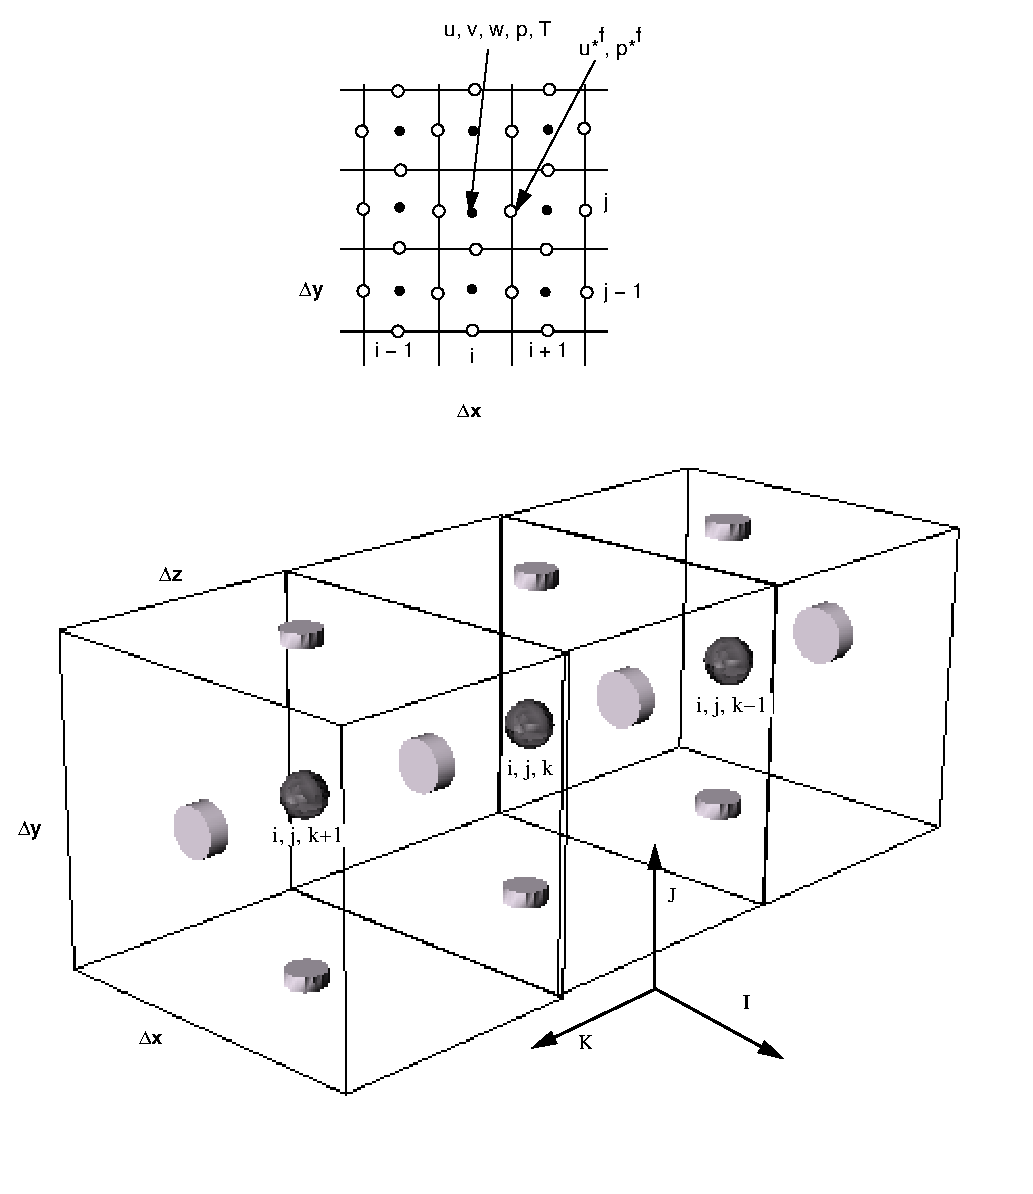
\includegraphics[scale=.85]{2dgrid.eps}
\caption{Two-Dimensional grid showing the location of the primary and auxiliary variables.}
\label{fig:2dgrid}
\end{figure}
%
%
%
%
%______________________________________________________________________
%  S  T  E  P     1  :   Equation of state
%______________________________________________________________________
\subsection{Step: \ref{step1}  \textsf{Discretized Equation of state}}
%
%
If the energy equation is not included then the discretized equations of state is
\begin{equation}
    \rho_{i,j,k} = \frac{p_{i,j,k}}{R T_{i,j,k}}
\end{equation}
%
%
where $R$ is the gas constant.  For constant specific heats and a ideal gas
the equations of state are
\begin{equation}
    p^{n}_{i,j,k} = (\gamma - 1) \rhonc_{i,j,k} e^{n^{c}}_{i,j,k} \quad \quad 
    \Tnc_{i,j,k} = \frac{(\gamma - 1)e^{n^{c}}_{i,j,k}}{R}
\end{equation}
%
%
%
%
%______________________________________________________________________
% Step 2A:  Discrete face-centered velocity
%______________________________________________________________________
\subsection{Step: \ref{step2}a  \textsf{Discretized Face-centered Velocity $\vec{U}^{\nadv^{*^{f}}}$}}
The discretized form of the face-centered velocity eq. (\ref{eq:ustar})
in the $x$, $y$ and $z$ directions is\\
%
%_______________________________
%  x direction
%_______________________________
\underline{\textsf{$x$-component}}
\begin{equation*}
    u^{\nadv^{*^f}}_{i,j,k,L}= \frac{(\rho \uvelnc)_{i-1,j,k} + (\rho \uvelnc)_{i,j,k}}{
    \rhonc_{i-1,j,k} + \rhonc_{i,j,k} }
-   \frac{ 2\delt(\pnnLc_{i,j,k} - \pnnLc_{i-1,j,k} ) }{\delx(\rhonc_{i-1,j,k} +  \rhonc_{i,j,k})}
    +  g_x \delt 
\end{equation*}
%
%_______________________________
%  x margin figure
%_______________________________
 \marginpar{\centering
 \includegraphics[width=\marginparwidth]{margin_figs_i.eps} }
 \\
%
%_______________________________
%  y direction
%_______________________________
\underline{\textsf{$y$-component}}
\begin{equation*}
    v^{\nadv^{*^f}}_{i,j,k,B}= \frac{(\rho \vvelnc)_{i,j,k} + (\rho \vvelnc)_{i,j-1,k}}{
    \rhonc_{i,j,k} + \rhonc_{i,j-1,k} }
-   \frac{ 2\delt(\pnnLc_{i,j,k} - \pnnLc_{i,j-1,k} ) }{\dely(\rhonc_{i,j,k} + \rhonc_{i,j-1,k})}
    + g_y \delt 
\end{equation*}
\\
%
%_______________________________
%  y margin figure
%_______________________________
 \marginpar{\centering
 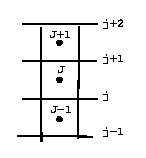
\includegraphics[height=0.75in]{margin_figs_j.eps}  }
\\
%
%_______________________________
%  z direction
%_______________________________
\underline{\textsf{$z$-component}}
\begin{equation*}
    w^{\nadv^{*^f}}_{i,j,k,BK}= \frac{(\rho \wvelnc)_{i,j,k-1} + (\rho \wvelnc)_{i,j,k}}{
    \rhonc_{i,j,k-1} + \rhonc_{i,j,k} }
-   \frac{ 2\delt(\pnnLc_{i,j,k}-\pnnLc_{i,j,k-1} ) }{\Delta{z}(\rhonc_{i,j,k-1} +      \rhonc_{i,j,k})}
+   g_z \delt 
\end{equation*}
%_______________________________
%  z margin figure
%_______________________________
 \marginpar{\centering
 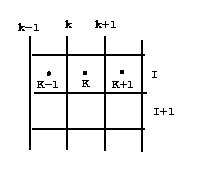
\includegraphics[width=\marginparwidth]{margin_figs_k.eps} }
\\
%
%______________________________________________________________________
%  S  T  E  P     2  :   Discretization of the change in the cell-centered equalibartion p
% pressure
%______________________________________________________________________
\subsection{Step: \ref{step2}b \textsf{Discretized change in the cell-centered equilibration pressure}}
This section needs to be filled in
%
%
%
%______________________________________________________________________
%    S  T  E  P     3  :   Discretized face-centered equalibartion p pressure
%______________________________________________________________________
\subsection{Step: \ref{step3} \textsf{Discretized change in the face-centered pressure}}


The discretized face-centered equilibration pressure eq. (\ref{eq:pstar}) is, \shortcite{ICE}\\
%_______________________________
%  x p*f faces 
%_______________________________
\underline{\textsf{$x$-direction}}
\begin{equation*}
    \pstar_{i,j,k,L} = \biggl{(}\frac{ \spvol_{i,j,k}\pnnLc_{i,j,k} + \spvol_{i-1,j,k} \pnnLc_{i-1,j,k}}{\spvol_{i,j,k} + \spvol_{i-1,j,k} } \biggr{)}
\end{equation*}
%
%_______________________________
%  x margin figure
%_______________________________
\normalmarginpar
\marginpar{\centering 
\includegraphics[width=0.75in]{margin_figs_i.eps} }
\\
%
%_______________________________
%  y p*f faces 
%_______________________________
\underline{\textsf{$y$-direction}}
\begin{equation*}
\pstar_{i,j,k,B} = \biggl{(}\frac{ \spvol_{i,j,k}\pnnLc_{i,j,k} + \spvol_{i,j-1,k}\pnnLc_{i,j-1,k}}
{\spvol_{i,j,k} + \spvol_{i,j-1,k} } \biggr{)} 
\end{equation*}
%
%
%_______________________________
%  y margin figure
%_______________________________
\marginpar{\centering
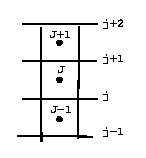
\includegraphics[height=0.75in]{margin_figs_j.eps}  }
\\
%
%_______________________________
%  z p*f faces 
%_______________________________
\underline{\textsf{$z$-direction}}
\begin{equation*}
\pstar_{i,j,k,BK} = \biggl{(}\frac{ \spvol_{i,j,k}\pnnLc_{i,j,k} + \spvol_{i,j,k-1}\pnnLc_{i,j,k-1}}
{\spvol_{i,j,k} + \spvol_{i,j,k-1} } \biggr{)}
\end{equation*}
%
%_______________________________
%  z margin figure
%_______________________________
 \marginpar{\centering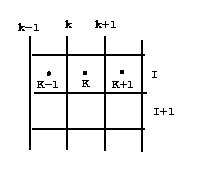
\includegraphics[width=0.75in]{margin_figs_k.eps} }
\\
%
%
%______________________________________________________________________
%  S  T  E  P     4  :   Source/Sink Terms
%______________________________________________________________________
\subsection{Step: \ref{step4} \textsf{Discretized Source/Sink Terms}}
Now performing the surface integrals, for a viscous compressible fluid
in Cartesian coordinates we get the following velocity source/sink terms.
Figure \ref{fig:vol_element} shows the diffusion of  the $x$-component of
momentum in and out of a control volume.
%
\begin{figure}
    \center
    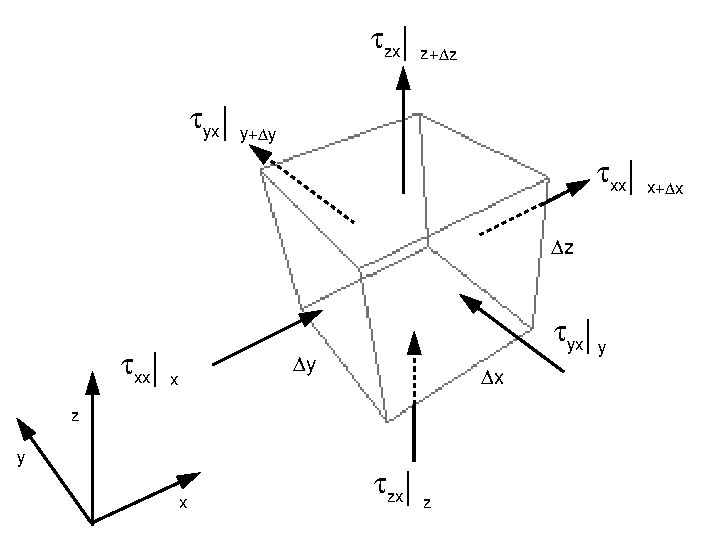
\includegraphics[scale=.85]{vol_element.eps}
    \caption{Volume element with arrows indicating the direction in which the x-component of momentum is transported through the surfaces.}
    \label{fig:vol_element}
\end{figure}
%
\\
% x component..............................
\underline{\textsf{$x$-component source terms}}\\
%
\begin{align*}
        \Delta{(m u)}^{\nadv}_{i,j,k}  &= 
        \delt( m^{n} u^n \dot{\alpha} )_{i,j,k}
-       \delt(   \pstar|_{i,j,k,R} - \pstar|_{i,j,k,L})\dely \delz\\
&   +   \delt\biggr(
    (   \tau^{f}_{xx}|_{i,j,k,R} - \tau^{f}_{xx}|_{i,j,k,L})\dely \delz
    +(  \tau^{f}_{yx}|_{i,j,k,T} - \tau^{f}_{yx}|_{i,j,k,B})\delx \delz\\
&   +(  \tau^{f}_{zx}|_{i,j,k,FR} - \tau^{f}_{zx}|_{i,j,k,BK})\delx \dely \biggl)
    +   m_{i,j,k}g_x\delt
\end{align*}
%
% y component..............................
\underline{\textsf{$y$-component source terms}}\\
%
\begin{align*}
        \Delta{(m v)^{\nadv}}  &= 
        \delt \langle m^{n} v^n \dot{\alpha} \rangle 
    -   \delt (   \pstar|_{i,j,k,T} - \pstar|_{i,j,k,B})\delx \delz\\
&   +   \delt \biggr(
    (   \tau^{f}_{xy}|_{i,j,k,R} - \tau^{f}_{xy}|_{i,j,k,L})\dely \delz
    +(  \tau^{f}_{yy}|_{i,j,k,T} - \tau^{f}_{yy}|_{i,j,k,B})\delx \delz\\
&   +(  \tau^{f}_{zy}|_{i,j,k,FR} - \tau^{f}_{zy}|_{i,j,k,BK})\delx \dely \biggl)
    +   m_{i,j,k}g_y\delt
\end{align*}
%
% z component..............................
\underline{\textsf{$z$-component source terms}}\\
%
\begin{align*}
        \Delta{(m w)^{\nadv}}   &= 
        \delt \langle m^{n} w^n \dot{\alpha} \rangle   
    -   \delt V^{n} 
    (   \pstar|_{j,k,k,FR} - \pstar|_{i,j,k,BK})\delx \dely\\
&   +   \delt\biggr(
    (   \tau^{f}_{xz}|_{i,j,k,R} - \tau^{f}_{xz}|_{i,j,k,L})\dely \delz
    +(  \tau^{f}_{yz}|_{i,j,k,T} - \tau^{f}_{yz}|_{i,j,k,B})\delx \delz\\
&   +(  \tau^{f}_{zz}|_{i,j,k,FR} - \tau^{f}_{zz}|_{i,j,k,BK})\delx \dely \biggl)
    +   m_{i,j,k}g_z\delt
\end{align*}
%
Now for the stress components we will discretize eqs. (\ref{eq:tau_xx} -
\ref{eq:tau_zx}) using second-order finite-difference centered representation
of the derivatives.  For a multimaterial problem we define an effective
viscosity across the right face of cell $i,j,k$
\begin{equation*}
\mu^{*^{f}}_{i,j,k,R} = \frac{2\mu_{i}\mu_{i+1}}{\mu_{i} + \mu_{i+1}}
\end{equation*}
All of the transport coefficients have this form.  For each face an edge
velocity, which is simply the average of the four nearest neighbors.
The naming convection is shown in fig. \ref{fig:edgevel}.
%
%
\begin{figure}
    \center
    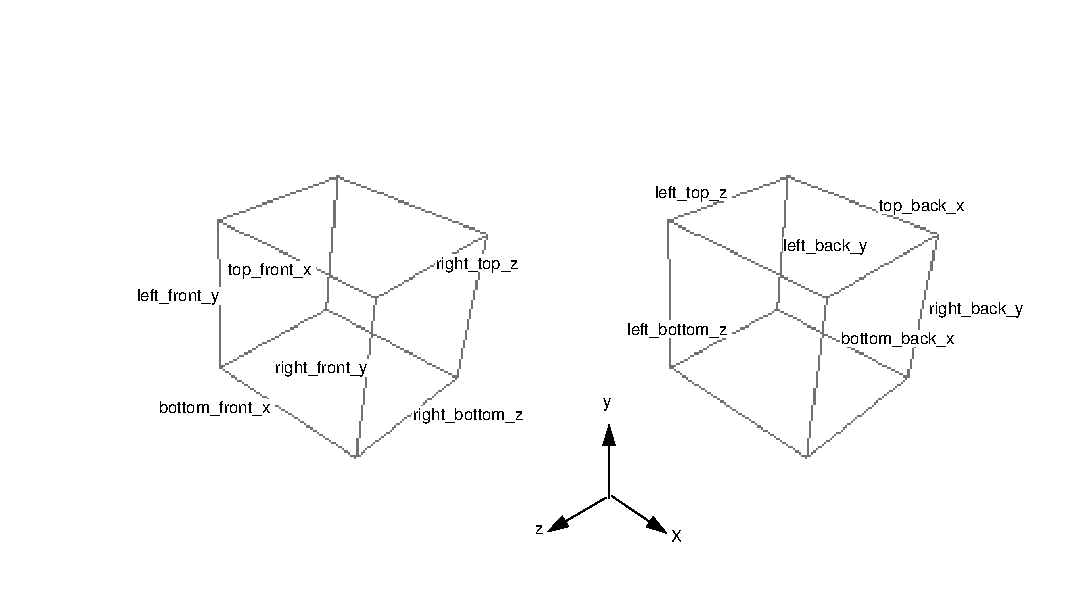
\includegraphics[scale=.8]{edge_velocity.eps}
    \caption{Naming convention for the edge velocities.}
    \label{fig:edgevel}
\end{figure}
%_______________________________
% Discrete tau_xx, tau_yy, tau_zz
%_______________________________
\begin{align*}
    \label{eq:tau_xx_d}
&       \tau^{f}_{xx}|_{left} =
    2   \mu^{*^{f}} \frac{ (\uvelnc_{i,j,k} - \uvelnc_{i-1,j,k}) }{ \delx }\\ 
&   -   \frac{2}{3}\mu^{*^{f}}\biggr(\frac{ (\uvelnc_{i,j,k} - \uvelnc_{i-1,j,k}) }{ \delx }
    +   \frac{ (v^{n^{e}}|^{left}_{top,z}   - v^{n^{e}}|^{left}_{bottom,z}) }{ \dely } 
    +   \frac{ (w^{n^{e}}|^{left}_{front,y} - w^{n^{e}}|^{left}_{back,y}) }{ \delz }\biggl)
\end{align*}
%
%_______________________________
%  x margin figure
%_______________________________
% \reversemarginpar
% \marginpar{\centering
% 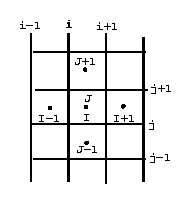
\includegraphics[width=\marginparwidth]{margin_figs_ij.eps} }
%
%
\begin{align*}
&       \tau^{f}_{xx}|_{right}= 
    2   \mu^{*^{f}} \frac{ (\uvelnc_{i+1,j,k} - \uvelnc_{i,j,k}) }{ \delx } \\ 
&   -   \frac{2}{3}\mu^{*^{f}}\biggr(\frac{ (\uvelnc_{i+1,j,k} - \uvelnc_{i,j,k}) }{ \delx }
    +   \frac{ (v^{n^{e}}|^{right}_{top,z}   - v^{n^{e}}|^{right}_{bottom,z}) }{ \dely } 
    +   \frac{ (w^{n^{e}}|^{right}_{front,y} - w^{n^{e}}|^{right}_{back,y}) }{ \delz }\biggl)
\end{align*}
%
%
\begin{align*}
    &   \tau^{f}_{yy}|_{bottom} = 
    2   \mu^{*^{f}} \frac{ (\vvelnc_{i,j,k} - \vvelnc_{i,j-1,k}) }{ \dely }\\ 
&   -   \frac{2}{3}\mu^{*^{f}}\biggr(\frac{ (u^{n^{e}}|^{bottom}_{right,z} - u^{n^{e}}|^{bottom}_{left,z}) }{ \delx }
    +   \frac{ (\vvelnc_{i,j,k} - \vvelnc_{i,j-1,k}) }{ \dely } 
    +   \frac{ (w^{n^{e}}|^{bottom}_{front,x} - w^{n^{e}}|^{bottom}_{back,x}) }{ \delz }\biggl )
\end{align*}
%
%
%_______________________________
%  y margin figure tau yy
%_______________________________
% \reversemarginpar
% \marginpar{\centering
% 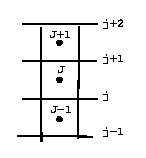
\includegraphics[width=\marginparwidth]{margin_figs_j.eps} }
%
%
\begin{align*}
&       \tau^{f}_{yy}|_{top} = 
    2   \mu^{*^{f}} \frac{ (\vvelnc_{i,j+1,k} - \vvelnc_{i,j,k}) }{ \dely } \\
&   -   \frac{2}{3}\mu^{*^{f}}\biggr(\frac{ (u^{n^{e}}|^{top}_{right,z} - u^{n^{e}}|^{top}_{left,z}) }{ \delx }
    +   \frac{ (\vvelnc_{i,j+1,k} - \vvelnc_{i,j,k}) }{ \dely } 
   +   \frac{ (w^{n^{e}}|^{top}_{front,x} - w^{n^{e}}|^{top}_{back,x}) }{ \delz }\biggl )
\end{align*}
%
\begin{align*}
&       \tau^{f}_{zz}|_{back} = 
    2   \mu^{*^{f}} \frac{ (\wvelnc_{i,j,k} - \wvelnc_{i,j,k-1}) }{ \delz }\\ 
&   -   \frac{2}{3}\mu^{*^{f}}\biggr(\frac{(u^{n^{e}}|^{back}_{right,y} - u^{n^{e}}|^{back}_{left,y}) }{ \delx }
    +   \frac{ (v^{n^{e}}|^{back}_{top,x}   - v^{n^{e}}|^{back}_{bottom,x}) }{ \dely } 
    +   \frac{ (\wvelnc_{i,j,k} - \wvelnc_{i,j,k-1}) }{ \delz }\biggl )
\end{align*}
%
%
%_______________________________
%  z margin figure tau zz
%_______________________________
% \reversemarginpar
% \marginpar{\centering
% 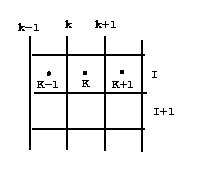
\includegraphics[width=\marginparwidth]{margin_figs_k.eps} }
%
%
\begin{align*}
&       \tau^{f}_{zz}|_{front} = 
    2   \mu^{*^{f}} \frac{ (\wvelnc_{i,j,k+1} - \wvelnc_{i,j,k}) }{ \delz }\\ 
&   -   \frac{2}{3}\mu^{*^{f}}\biggr(\frac{(u^{n^{e}}|^{front}_{right,y} - u^{n^{e}}|^{front}_{left,y}) }{ \delx }
    +   \frac{ (v^{n^{e}}|^{front}_{top,x}   - v^{n^{e}}|^{front}_{bottom,x}) }{ \dely }  
   +   \frac{ (\wvelnc_{i,j,k+1} - \wvelnc_{i,j,k}) }{ \delz }\biggl )
\end{align*}
%
%_______________________________
% discrete tau_xy, tau_xz, tau_yx
%_______________________________
\begin{equation*}
    \tau^{f}_{xy}|_{left} = 
    \mu^{*^{f}} \biggr(\frac{ (u^{n^{e}}|^{left}_{top,z} - u^{n^{e}}|^{left}_{bottom,z}) }{ \dely } 
+   \frac{ (\vvelnc_{i,j,k} - \vvelnc_{i-1,j,k}) }{ \delx } \biggl)
\end{equation*}
%
%
\begin{equation*}
    \tau^{f}_{xy}|_{right} = 
    \mu^{*^{f}} \biggr(\frac{ (u^{n^{e}}|^{right}_{top,z} - u^{n^{e}}|^{right}_{bottom,z}) }{ \dely } 
+   \frac{ (\vvelnc_{i+1,j,k} - \vvelnc_{i,j,k}) }{ \delx } \biggl)
\end{equation*}
%
%
\begin{equation*}
    \tau^{f}_{xz}|_{left} =
    \mu^{*^{f}} \biggr(\frac{ (u^{n^{e}}|^{left}_{front,y} - u^{n^{e}}|^{left}_{back,y}) }{ \delz } 
+   \frac{ (\wvelnc_{i,j,k} - \wvelnc_{i-1,j,k}) }{ \delx }\biggl )
\end{equation*}
%
%
\begin{equation*}
    \tau^{f}_{xz}|_{right} =
    \mu^{*^{f}} \biggr(\frac{ (u^{n^{e}}|^{right}_{front,y} - u^{n^{e}}|^{right}_{back,y}) }{ \delz }
+   \frac{ (\wvelnc_{i+1,j,k} - \wvelnc_{i,j,k}) }{ \delx } \biggl )
\end{equation*}
%
%
\begin{equation*}
    \tau^{f}_{yx}|_{bottom} = 
    \mu^{*^{f}} \biggr(\frac{ (\uvelnc_{i,j,k} - \uvelnc_{i,j-1,k}) }{ \dely } 
+   \frac{ (v^{n^{e}}|^{bottom}_{right,z} - v^{n^{e}}|^{bottom}_{left,z}) }{ \delx } \biggl)
\end{equation*}
%
%
\begin{equation*}
    \tau^{f}_{yx}|_{top} = 
    \mu^{*^{f}} \biggr(\frac{ (\uvelnc_{i,j+1,k} - \uvelnc_{i,j,k}) }{ \dely } 
+   \frac{ (v^{n^{e}}|^{top}_{right,z} - v^{n^{e}}|^{top}_{left,z}) }{ \delx } \biggl)
\end{equation*}
%
%_______________________________
% discrete tau_yz, tau_zx, tau_zy
%_______________________________
\begin{equation*}
    \tau^{f}_{yz}|_{bottom} = 
    \mu^{*^{f}} \biggr(\frac{ (v^{n^{e}}|^{bottom}_{front,x}   - v^{n^{e}}|^{bottom}_{back,x}) }{ \delz } 
+   \frac{ (\wvelnc_{i,j,k} - \wvelnc_{i,j,k-1}) }{ \dely } \biggl)
\end{equation*}
%
\begin{equation*}
    \tau^{f}_{yz}|_{top} = 
    \mu^{*^{f}} \biggr(\frac{ (v^{n^{e}}|^{top}_{front,x}   - v^{n^{e}}|^{top}_{back,x}) }{ \delz } 
+   \frac{ (\wvelnc_{i,j+1,k} - \wvelnc_{i,j,k}) }{ \dely } \biggl)
\end{equation*}
%
\begin{equation*}
    \tau^{f}_{zx}|_{back} =
    \mu^{*^{f}} \biggr(\frac{ (\uvelnc_{i,j,k} - \uvelnc_{i,j,k-1}) }{ \delz } 
+   \frac{  (w^{n^{e}}|^{back}_{right,y} - w^{n^{e}}|^{back}_{left,y})  }{ \delx }\biggl )
\end{equation*}
%
\begin{equation*}
    \tau^{f}_{zx}|_{front} =
    \mu^{*^{f}} \biggr( \frac{ (\uvelnc_{i,j,k+1} - \uvelnc_{i,j,k}) }{ \delz }
+   \frac{ (w^{n^{e}}|^{front}_{right,y} - w^{n^{e}}|^{front}_{left,y}) }{ \delx } \biggl )
\end{equation*}
%
%
\begin{equation*}
    \tau^{f}_{zy}|_{back} = 
    \mu^{*^{f}} \biggr(\frac{ (\vvelnc_{i,j,k} - \vvelnc_{i,j,k-1}) }{ \delz } 
+   \frac{ (w^{n^{e}}|^{back}_{top,x} - w^{n^{e}}|^{back}_{bottom,x}) }{ \dely } \biggl)
\end{equation*}
%
\begin{equation*}
    \tau^{f}_{zy}|_{front} = 
    \mu^{*^{f}} \biggr(\frac{ (\vvelnc_{i,j,k+1} - \vvelnc_{i,j,k}) }{ \delz } 
+   \frac{ (w^{n^{e}}|^{front}_{top,x} - w^{n^{e}}|^{front}_{bottom,x}) }{ \dely } \biggl)
\end{equation*}
%
%
%_______________________________
% Energy equation source terms
%_______________________________
\underline{\textsf{Energy equation source terms}}\\
\begin{equation}
    \Delta( m e)^{\nadv}_{ijk}  = \delt (\nabla \cdot \vec{U})_{ijk}
\end{equation}
%
%
%
%
%______________________________________________________________________
%  S  T  E  P     5  :   Lagrangian Values
%______________________________________________________________________
\subsection{Step: \ref{step5}  \textsf{ Discretized Lagrangian $\rho^{L}, (m\vec{U})^{L}, e^{L}$}}

The equations for calculating the Lagrangian contribution of the total mass,
momentum, and energy are\\
\\
%
%
%_______________________________volume Lagr.
\underline{\textsf{Mass:}}\\
\begin{equation}
    \massnnLIJK = \rhonIJK \VnIJK + 
\overbrace{  \Delta{(m_{m})}^{\nadv}_{i,j,k}  }^{\text{source/sink}}  
\end{equation}
%
%
%
%_______________________________momentum Lagr
\underline{\textsf{Momentum:}}\\

\begin{equation}
    (mu)^{\nadv^{L}}_{i,j,k} = (mu)^{n^{c}}_{i,j,k} 
    -   \overbrace{ \uncIJK \Delta{ (m) }^{\nadv}_{i,j,k}}^{ \text{\pboxsmall{source/sink due to phase change}}} 
    +   \overbrace{   \Delta{ (mu) }^{\nadv}_{i,j,k}    }^{  \text{source/sink}  }
\end{equation}
%
%
\begin{equation}
    (mv)^{\nadv^{L}}_{i,j,k} = (mv)^{n^{c}}_{i,j,k} 
    -   \overbrace{ \vncIJK \Delta{ (m) }^{\nadv}_{i,j,k}}^{ \text{\pboxsmall{source/sink due to phase change}}} 
    +   \overbrace{   \Delta{ (mv) }^{\nadv}_{i,j,k}    }^{  \text{source/sink}  }
\end{equation}
%
%
\begin{equation}
    (mw)^{\nadv^{L}}_{i,j,k} = (mw)^{n^{c}}_{i,j,k} 
    -   \overbrace{ \wncIJK \Delta{ (m) }^{\nadv}_{i,j,k}}^{ \text{\pboxsmall{source/sink due to phase change}}} 
    +   \overbrace{   \Delta{ (mw) }^{\nadv}_{i,j,k}    }^{  \text{source/sink}  }
\end{equation}   
%
%
%_______________________________energy Lagr
\underline{\textsf{Energy: (The contribution from the kinetic energy is currently missing)}}\\
%
\begin{equation}
     e^{L^{\nadv}}_{i,j,k}= e^n_{i,j,k}  - \overbrace{  e^n_{i,j,k} \Delta{(m)}^{\nadv}_{i,j,k}}^{\text{\pboxsmall{source/sink due to phase change} }  } +
    \overbrace{  \Delta{ (m e)^{\nadv}_{i,j,k}  }  }^{  \text{source/sink}  }
\end{equation}
\\
%
where $e^n= (c_{v}T)^n_.$\\
%
%
%
%
%______________________________________________________________________
%  S  T  E  P     6  :   Advection
%______________________________________________________________________
\subsection{Step: \ref{step6}  \textsf{Discretized Advection Operator}}
\textbf{ This section is out of date.  We do not use the corner coupling volumes (2 and 3)}

Below is the advection operator, eq. (\ref{eq:advect.main}), with the
influx and outflux summation terms expanded, assuming $u~=~v~=~ 1.0$,
see Fig(\ref{Fig:flux_vol_1}).
%
%
\begin{multline}
    -\delt\text{Advection}( (q), \ustar) = \\
    \overbrace{- \biggl{[} 
    \langle{q}\rangle_{1,i,j} \Delta{V}_{1,i,j}  
+   \langle{q}\rangle_{2,i,j} \Delta{V_{2,i,j}}
+   \langle{q}\rangle_{3,i,j} \Delta{V_{3,i,j}}
+   \langle{q}\rangle_{4,i,j} \Delta{V_{4,i,j}} \biggr{]} }^{outflux}           \\
    \overbrace{+ \biggl{[} 
    \langle{q}\rangle_{1,i,j} \Delta{V}_{1,i,j-1}  
+   \langle{q}\rangle_{2,i,j} \Delta{V_{2,i-1,j-1}}
+   \langle{q}\rangle_{3,i,j} \Delta{V_{3,i-1,j-1}}
+   \langle{q}\rangle_{4,i,j} \Delta{V_{4,i-1,j}} \biggr{]} }^{influx}           \\
\end{multline}
%
%
The discretized equation for outflux of $q$ eq. (\ref{eq:qoutflux}) is \\
%
%
\begin{align}
    \langle{q}\rangle_{1,i,j,k} = q_{i,j,k} 
+   \pd{q_{i,j,k}}{x} \mathbf{r_{x,1}}
+   \pd{q_{i,j,k}}{y} \mathbf{r_{y,1}} \\
    \label{eq:discrete.qoutflux1}
    \langle{q}\rangle_{2,i,j,k} = q_{i,j,k} 
+   \pd{q_{i,j,k}}{x} \mathbf{r_{x,2}}
+   \pd{q_{i,j,k}}{y} \mathbf{r_{y,2}}  \\
    \label{eq:discrete.qoutflux2}
    \langle{q}\rangle_{3,i,j,k} = q_{i,j,k} 
+   \pd{q_{i,j,k}}{x} \mathbf{r_{x,3}}
+   \pd{q_{i,j,k}}{y} \mathbf{r_{y,3}}   \\
    \label{eq:discrete.qoutflux3}
    \langle{q}\rangle_{4,i,j,k} = q_{i,j,k} 
+   \pd{q_{i,j,k}}{x} \mathbf{r_{x,4}}
+   \pd{q_{i,j,k}}{y} \mathbf{r_{y,4}}   
\end{align}
    \label{eq:discrete.qoutflux4}
%
%
where the centroids for each outflux volume are shown below.  The differencing
scheme used to approximate the gradients of $q$ is discussed in the appendix.
%
%
Listed below are the equations for the outflow volume fluxes for cell $i,j$, at
time $t$, and the the associated centroids, Fig. (\ref{Fig:flux_vol_1})  Note
that the equations for the centroids vary depending on the velocity direction.
%__________________________________
%   Courant Number
%___________________________________
The lengths $B$ and $H$ used in the equations below are given by $|u * \delt|$
and $|v * \delt|$ respectively and $l_{1} = \delx - B$ and $l_{2} = \dely - H$
The Courant numbers $\sigma_{x}=\frac{ u \delt}{\delx}$ and $\sigma_{y} =
\frac{ v \delt}{\dely}$ must satisfy $\sigma_x< 1$ and $\sigma_y < 1$.
\\
\\
%______________________________________________________________________
%               OUTFLOW FLUXES
%_______________________________________________________________________
\underline{$(\nearrow, u > 0, v > 0)$, cell $(i, j)$, Fig. (\ref{Fig:flux_vol_1}a)}
\\
\[  \underset{outflow}{\Delta V_{i,j}}      = \delV_1 + \delV_2 + \delV_3 + \delV_4  \]
%
%
\[  \rr_{x,4} = l_1 + \frac{B}{2} -\XCC,   \quad   \rr_{y,4} = \frac{l_2}{2} - \YCC,   
    \quad
    \rr_{x,1} = \frac{l_1}{2} - \XCC,      \quad   \rr_{y,1} = l_2  + \frac{H}{2} - \YCC \]
%
%
\[  \rr_{x,2} = l_1 + \frac{B}{3} - \XCC,   \quad   \rr_{y,2} = l_2 + \frac{2H}{3} - \YCC,
    \quad                              
    \rr_{x,3} = l_1 + \frac{2B}{3} - \XCC,  \quad   \rr_{y,3} = l_2 + \frac{H}{3} - \YCC\]
%
%
\\
\\
%__________________________________
% U > 0, V < 0
%___________________________________
\underline{$(\searrow, u > 0, v < 0)$, cell $(i, j)$, Fig. (\ref{Fig:flux_vol_1}b)}
\\
%
%
\[  \rr_{x,4} = l_1 + \frac{B}{2} - \XCC,   \quad   \rr_{y,4} = H + \frac{l_2}{2} - \YCC,   
    \quad
    \rr_{x,1} = \frac{l_1}{2} - \XCC,       \quad   \rr_{y,1} = \frac{H}{2} - \YCC \]
%
%
\[  \rr_{x,2} = l_1 + \frac{B}{3} - \XCC,   \quad   \rr_{y,2} = \frac{H}{3} - \YCC,
    \quad                              
    \rr_{x,3} = l_1 + \frac{2B}{3} - \XCC,  \quad   \rr_{y,3} = \frac{2H}{3} - \YCC\]
%
%
\\
\\
\underline{$(\nwarrow, u < 0, v > 0)$, cell $(i, j)$, Fig. (\ref{Fig:flux_vol_1}c)}
\\
%
%
\[  \rr_{x,4} = \frac{B}{2} - \XCC,            \quad   \rr_{y,4} = \frac{l_2}{2} - \YCC,   
    \quad
    \rr_{x,1} = B + \frac{l_1}{2} - \XCC,      \quad   \rr_{y,1} = l_2  + \frac{H}{2} - \YCC \]
%
%
\[  \rr_{x,2} = \frac{2B}{3} - \XCC,           \quad   \rr_{y,2} = l_2 + \frac{2H}{3} - \YCC,
    \quad                              
    \rr_{x,3} = \frac{B}{3} - \XCC,            \quad   \rr_{y,3} = l_2 + \frac{H}{3} - \YCC\]
%
%
%
\\
\\
\underline{$(\swarrow, u < 0, v < 0)$, cell $(i, j)$, Fig. (\ref{Fig:flux_vol_1}d)}
\\
%
%
\[  \rr_{x,4} = \frac{B}{2} - \XCC,         \quad   \rr_{y,4} = H + \frac{l_2}{2} - \YCC,   
    \quad
    \rr_{x,1} = B + \frac{l_1}{2} - \XCC,   \quad   \rr_{y,1} = \frac{H}{2} - \YCC \]
%
%
\[  \rr_{x,2} = \frac{2B}{3} - \XCC,        \quad   \rr_{y,2} = \frac{H}{3} - \YCC,
    \quad                              
    \rr_{x,3} = \frac{B}{3} - \XCC,         \quad   \rr_{y,3} = \frac{2H}{3} - \YCC\]
%
%
In a compact form the outflow volume centroids of cell $i, j$ can be written as
%__________________________________
%  r_4 OUTFLOW
%___________________________________*/
\begin{alignat}{3}
    &\rr_{x,4} = C_4 + \frac{B}{2} - \XCC           \quad&
    \begin{cases}
        \nearrow \searrow, \text{or}~u >0,  \quad   C_4 = l_1;     &   \text{case 1}   
 \\
        \nwarrow \swarrow, \text{or}~u <0,  \quad   C_4 = 0;       &   \text{case 2}
    \end{cases}
%
\\
%
    &\rr_{y,4} = C_4 + \frac{l_2}{2} - \YCC         \quad&
    \begin{cases}
        \nearrow \nwarrow, \text{or}~v >0,   \quad   C_4 = 0;      &   \text{case 3} 
 \\
        \searrow \swarrow, \text{or}~v <0,   \quad   C_4 = H;      &   \text{case 4}
    \end{cases}
\end{alignat}
%
%
%__________________________________
%  r_1 OUTFLOW
%___________________________________*/
\begin{alignat}{3}
    &\rr_{x,1} = C_1 + \frac{l_1}{2} - \XCC         \quad&
    \begin{cases}
        \nearrow \searrow, \text{or}~u >0,  \quad   C_1 = 0;       &   \text{case 1}   
 \\
        \nwarrow \swarrow, \text{or}~u <0,  \quad   C_1 = B;       &   \text{case 2}
    \end{cases}
%
\\
%
    &\rr_{y,1} = C_1 + \frac{H}{2} - \YCC           \quad&
    \begin{cases}
        \nearrow \nwarrow, \text{or}~v >0,   \quad   C_1 = l_2;    &   \text{case 3} 
 \\
        \searrow \swarrow, \text{or}~v <0,   \quad   C_1 = 0;      &   \text{case 4}
    \end{cases}
\end{alignat}
%
%
%__________________________________
%  r_2 OUTFLOW
%___________________________________*/
\begin{alignat}{3}
    &\rr_{x,2} = C_2 + \alpha\frac{B}{3} - \XCC     \quad&
    \begin{cases}
        \nearrow \searrow, \text{or}~u >0,\quad C_2 = l_1;  \quad   \alpha = 1  &   \text{case1}
 \\
        \nwarrow \swarrow, \text{or}~u <0,\quad C_2 = 0;    \quad   \alpha = 2  &   \text{case2}
    \end{cases}
%
\\
%
    &\rr_{y,2} = C_2 + \alpha\frac{H}{3} - \YCC     \quad&
    \begin{cases}
        \nearrow \nwarrow,\text{or}~v >0, \quad C_2 = l_2; \quad   \alpha = 2   &   \text{case3}
 \\
        \searrow \swarrow,\text{or}~v <0, \quad C_2 = 0;   \quad   \alpha = 1   &   \text{case4}
    \end{cases}
\end{alignat}
%
%
%__________________________________
%  r_3 OUTFLOW
%___________________________________*/
\begin{alignat}{3}
    &\rr_{x,3} = C_3 + \alpha\frac{B}{3} - \XCC     \quad&
    \begin{cases}
        \nearrow \searrow, \text{or}~u >0,\quad C_3 = l_1;  \quad   \alpha = 2  &   \text{case1}
 \\
        \nwarrow \swarrow, \text{or}~u <0,\quad C_3 = 0;    \quad   \alpha = 1  &   \text{case2}
    \end{cases}
%
\\
%
    &\rr_{y,3} = C_3 + \alpha\frac{H}{3} - \YCC     \quad&
    \begin{cases}
        \nearrow \nwarrow,\text{or}~v >0, \quad C_3 = l_2; \quad   \alpha = 1   &   \text{case3}
 \\
        \searrow \swarrow,\text{or}~v <0, \quad C_3 = 0;   \quad   \alpha = 2   & \text{case4}
    \end{cases}
\end{alignat}
%
%
\\
%______________________________________________________________________
%               INFLOW FLUXES
%_______________________________________________________________________
The equations for the inflow volume fluxes to the surrounding cells and
the associated centroids are shown below. Note the coordinate system for
each of the surrounding cells is the cell centroid of that particular cell,
$\delx/2, \dely/2$.
%
%
\begin{figure}
    \center
    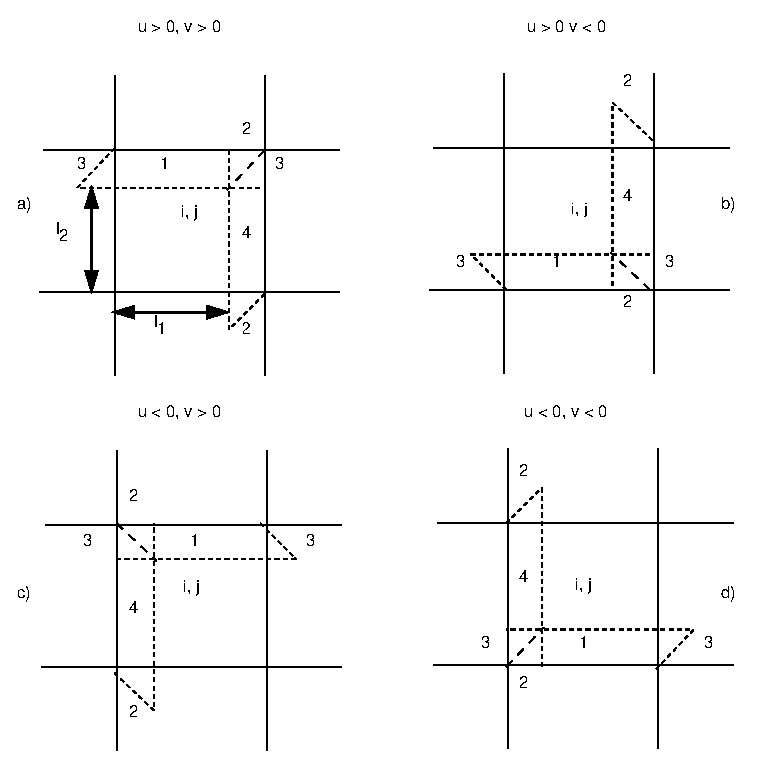
\includegraphics{advect_flux_vol_1.eps}
    \caption{Cell (i, j) with outflow fluxes shown at time $t$}
    \label{Fig:flux_vol_1}
\end{figure}
%
%
\begin{figure}
    \center
    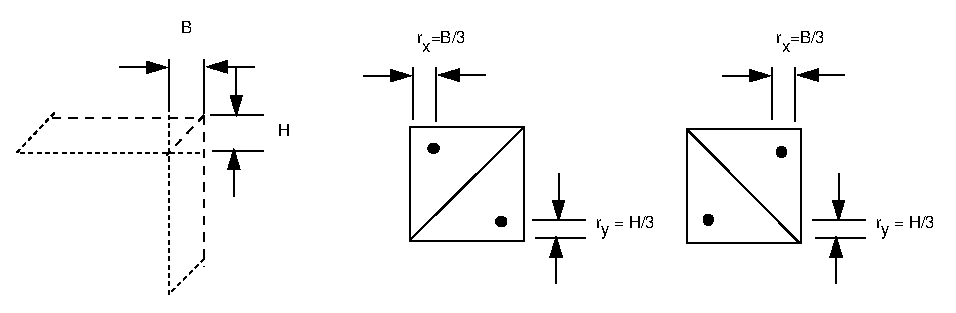
\includegraphics{advect_flux_vol_2.eps}
    \caption{outflow fluxes shown at time $t$}
    \label{Fig:flux_vol_2}
\end{figure}
%
%
\\
\\
\underline{$(\nearrow, u > 0, v > 0)$, contribution from cell $(i, j)$, Fig. (\ref{Fig:flux_vol_1}a)}
\\
\[  \underset{inflow}{\Delta V_{i+1,j}}      = \delV_{4,i,j} 
    \quad ; \quad 
    \underset{inflow}{\Delta V_{i+1,j+1}}    = \delV_{2,i,j} + \delV_{3,i,j}
    \quad ; \quad 
    \underset{inflow}{\Delta V_{i,j+1}}      = \delV_{1,i,j}\]
%
\\
\\
%__________________________________
% U > 0, V < 0
%___________________________________
\underline{$(\searrow, u > 0, v < 0)$, contribution from cell $(i, j)$, Fig. (\ref{Fig:flux_vol_1}b)}
\\
\[  \underset{inflow}{\Delta V_{i+1,j}}      = \delV_{4,i,j}
    \quad ; \quad 
    \underset{inflow}{\Delta V_{i+1,j-1}}    = \delV_{2,i,j} + \delV_{3,i,j}
    \quad ; \quad 
    \underset{inflow}{\Delta V_{i,j-1}}      = \delV_{1,i,j}\]
%
%
\\
\\
\underline{$(\nwarrow, u < 0, v > 0)$, contribution from cell $(i, j)$, Fig. (\ref{Fig:flux_vol_1}c)}
\\
\[  \underset{inflow}{\Delta V_{i-1,j}}      = \delV_{4,i,j}  
    \quad ; \quad 
    \underset{inflow}{\Delta V_{i-1,j+1}}    = \delV_{2,i,j} + \delV_{3,i,j}
    \quad ; \quad 
    \underset{inflow}{\Delta V_{i,j+1}}      = \delV_{1,i,j}\]
%
\\
\\
\underline{$(\swarrow, u < 0, v < 0)$, contribution from cell $(i, j)$, Fig. (\ref{Fig:flux_vol_1}d)}
\\
\[  \underset{inflow}{\Delta V_{i-1,j}}      = \delV_{4,i,j}  
    \quad ; \quad 
    \underset{inflow}{\Delta V_{i-1,j-1}}    = \delV_{2,i,j} + \delV_{3,i,j}
    \quad ; \quad 
    \underset{inflow}{\Delta V_{i,j-1}}      = \delV_{1,i,j}\]
%
%
where,
\[  \delV_3 = \frac{BH}{2}      \quad;  \quad  \delV_2 = \frac{BH}{2}\]
\[  \delV_4 = (\dely - H)(B)            \quad;  \quad  \delV_1 = (\delx - B)(H)\]
\[  l_2 = \dely - H             \quad;  \quad   l_1 = \delx - B \]
%
%
%
%__________________________________
%   vertex values of q
%___________________________________
\subsection{Vertex values of $q_v$}

The discretized equations for the vertex values of $q$ interpolated by
eq. (\ref{eq:vertex}) in 2-dimensions is, Fig. (\ref{Fig:cell}).
%
%
\begin{figure}
    \center
    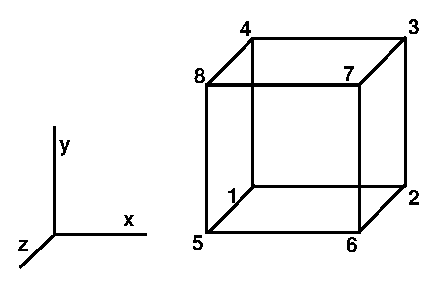
\includegraphics{advect_cell_vertices.eps}
    \caption{Schematic of a cell with vertices labeled}
    \label{Fig:cell}
\end{figure}
%
%
\begin{alignat}{2}
    &q^{1} = q_{ijk} 
+   \pd{q_{ijk}}{x}(- \frac{\delx}{2}) 
&+  \pd{q_{ijk}}{y}(- \frac{\dely}{2})
    \label{eq:vertex1} 
%
\\
%
    &q^{2} = q_{ijk} 
+   \pd{q_{ijk}}{x}(\frac{\delx}{2}) 
&+  \pd{q_{ijk}}{y}(- \frac{\dely}{2}) 
%
\\
%
    &q^{3} = q_{ijk} 
+   \pd{q_{ijk}}{x}(\frac{\delx}{2}) 
&+  \pd{q_{ijk}}{y}(\frac{\dely}{2}) 
%
\\
%
    &q^{4} = q_{ijk} 
+   \pd{q_{ijk}}{x}(-\frac{\delx}{2}) 
&+   \pd{q_{ijk}}{y}(\frac{\dely}{2}) 
    \label{eq:vertex4}
\end{alignat}
%
%
\textbf{Note: a simple approach may be to use} 
\\
$q^{1} = 0.25( q_{ijk} + q_{i-1jk} + q_{i-1j-1k} + q_{ij-1k} )$\\
\\
\\
%__________________________________
%   Gradients
%___________________________________
The gradients of $q$ are approximated by second-order finite difference
%
%
\begin{equation}
    \pd{q}{x} = \frac{q_{i+1} - q_{i-1}}{2\delx}
\end{equation}
%
%
\begin{equation}
    \pd{q}{y} = \frac{q_{j+1} - q_{j-1}}{2\dely}
\end{equation}
%
%
%
%
%______________________________________________________________________
%  S  T  E  P     7  :     Discretized time advanced equations 
%______________________________________________________________________
\subsection{ Step: \ref{step7}  \textsf{Discretized Time Advanced Equations}}
Below is the discretized equations for the time advanced mass, momentum and
internal energy, eq. (\ref{eq:rho^n+1} - \ref{eq:T^n+1})  \\
%
\begin{equation}
(m)^{n+1}_{i,j,k} = \massnnL_{ijk} - \delt\text{Advection}(\rho^{\nadv^{L}}_{i,j,k}\ustar)
\end{equation}
%
\begin{equation}
(mu)^{n+1}_{i,j,k} =(m u)^{\nadv^{L}}_{i,j,k} - \delt\text{Advection}( (\rho u)^{\nadv^{L}}_{i,j,k},\ustar)
\end{equation}
%
\begin{equation}
(mv)^{n+1}_{i,j,k} =(m v)^{\nadv^{L}}_{i,j,k} - \delt\text{Advection}( (\rho v)^{\nadv^{L}}_{i,j,k}, \ustar)
\end{equation}
%
\begin{equation}
(mw)^{n+1}_{i,j,k} =(m w)^{\nadv^{L}}_{i,j,k} - \delt\text{Advection}( (\rho w)^{\nadv^{L}}_{i,j,k}, \ustar)
\end{equation}
%
\begin{equation}
(me)^{n+1}_{i,j,k} =(m c_v T)^{\nadv^{L}}_{i,j,k} - \delt\text{Advection}( (\rho c_v T)^{\nadv^{L}}_{i,j,k}, \ustar)
\end{equation}
\par
%
%
%
%
\iffalse
%______________________________________________________________________
% description here
%______________________________________________________________________
\section{\textsf{Boundary Conditions and Data Dependencies}}
Dirichlet, Neumann and LODI type boundary conditions are currently available.\\
\underline{Initial Conditions}\\
The primary dependent variables $u, v, w \rho, T$ must be initialized at
the start of the calculation.  Initial conditons must be set in the entire
computational domain including the ghostcells.  The initial conditions on
the thermodynamic variables $\rho, T$ in the ghostcells also serve as default
boundary condtions, since their values in these cells remain unchanged unless
they are changed by imposing the boundary conditions.\\

\underline{Boundary Conditions}\\
The correct specification of boundary conditions is essential to the success
of a calculation.  Their specification is the most demanding and error-prone
task involved in setting up a problem, and requires conscientiousness and
understanding on the part of the user.  A number of different yet interrelated
considerations are involved.

\underline{Physical and Numerical Boundary Conditions}\\
The partial differential equations require certain physical boundary conditions
to determine a solution uniquely.  However, finite-difference equations
usually require additional boundary conditons that would overspecify the
differential problem.  ICE requires that boundary values be set for the
velocity components $u$ and $v$ and the thermodynamic variables $\rho, e,
p, T$.  In a given problem and at a boundary point, some of these boundary
values will be determined by the physical boundary conditions.  The others
should be set to allow the variables in question to ``float;" i.e., to adjust
themselves to the developing solution approximately as they would in the
differential problem.  Proper sets of boundary conditons on different types
of boundaries are summarized in the following.

\underline{Thermodynamic Consistency}\\
The thermodynamic variables $\rho, e, p, T$ are not all independent, and
their values in the ghostcells should set self-consistently, so that the
state relations are statisfied.  These consistency conditions must be borne
in mind when setting ``floating" bounday conditions, because they imply that
the floating variables cannot always float independently.  Depending on the
physical boundary conditions, however, some of the floating boundary values
may not influence the solution, and in such cases complete self-consistency
is not necessary.

\underline{``Floating" boundary Conditions}\\
Thre are two simple ways of allowing a boundary value to ``float."  The first
and simplest is the ``zero-slope" method.  In this method, the value of a
floating thermodynamic variable in an ghost cell is set equal to the value
of that variable in the adjacent interior cell.....

The second method for allowing a boundary value to float is the
``extrapolation" method, in which the value of a floating thermodynamic
variable in a ghostcell is obtained by extrapolation from the values
in the adjacent two layers of interior cells.  The value of a floating
velocity...............

\underline{Boundary Conditions at a Free-Slip Boundary}\\
The primary physical boundary condition in this case is that the velocity
vector on the boundary is parallel to the boundary..........

In this case the thermodynamic variables $\rho$ and $p$ in the ghostcells
are then set by the extrapolation method.  Thermal and diffusion fluxes are
ordinarily zero on a free-slip boundary.................

\subsection{Data dependencies}
Figures \ref{fig:boundarycondpg1} - \ref{fig:boundarycondpg4} show the data
dependency on ghostcell data in each of the main comutational steps described
above.  For example, in step 1: equation of state, the cell-centered pressure
depends on the cell-centered density, temperature and the ideal gas properties.
In Fig(\ref{fig:boundarycondpg1}) note that both the X and O are located inside
of each of the corner cells. In step 3, compute the face-centered pressure,
you'll see that each press\_FC depends on the cell-centered density and
pressure on either side of that face.  Note the variable $q$ shown in Fig
(\ref{fig:boundarycondpg3}) is equivalent to $\rho,~\rho u,~\rho v,~\rho
w,~\rho c_vT.$  The gray boxes represent the comutational domain and the
surrounding layer of cells are the ghostcells.


It is assumed that the face-centered values along the outer edge of the
ghostcell layer are equal to the cell-centered values, so that
\begin{align}
    (u,v,w)^{*^{f}}_{{imax,j,k,R}} &= (u,v,w)^{n^{c}}_{imax,j,k};   \quad  
    (u,v,w)^{*^{f}}_{{imin,j,k,L}} = (u,v,w)^{n^{c}}_{imin,j,k}     \notag \\
    (u,v,w)^{*^{f}}_{{i,jmax,k,T}} &= (u,v,w)^{n^{c}}_{i,jmax,k};   \quad  
    (u,v,w)^{*^{f}}_{{i,jmin,k,B}} = (u,v,w)^{n^{c}}_{i,jmin,k}     \notag \\
    p^{*^{f}}_{{imax,j,k,R}} &= p^{n^{c}}_{imax,j,k}                \notag \\     
    p^{*^{f}}_{{i,jmin,k,B}} &= p^{n^{c}}_{i,jmin,k}                \notag 
\end{align}


In calculating the gradient limiter in the corner ghostcells the max. and
min. values of the surrounding cell-centered data is needed.  Since we don't
have data that lies outside of the ghostcells data from four cells nearest
the corner of interest is used, see Fig (\ref{fig:boundarycondpg3}).
%
%
\begin{figure}
    \center
    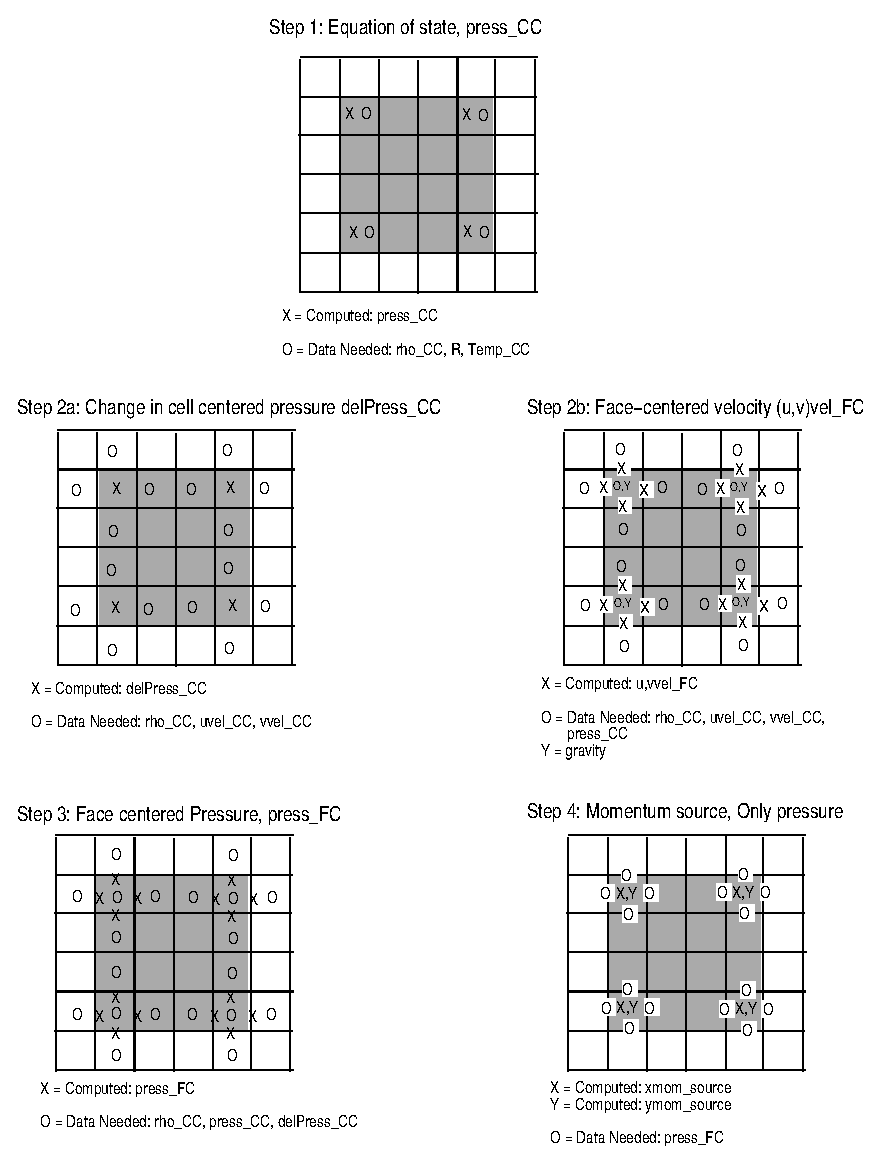
\includegraphics{boundarycond_pg1.eps}
    \caption{The dependency on ghost cell data for the computations in steps 1 - 4}
    \label{fig:boundarycondpg1}
\end{figure}
%
%
\begin{figure}
    \center
    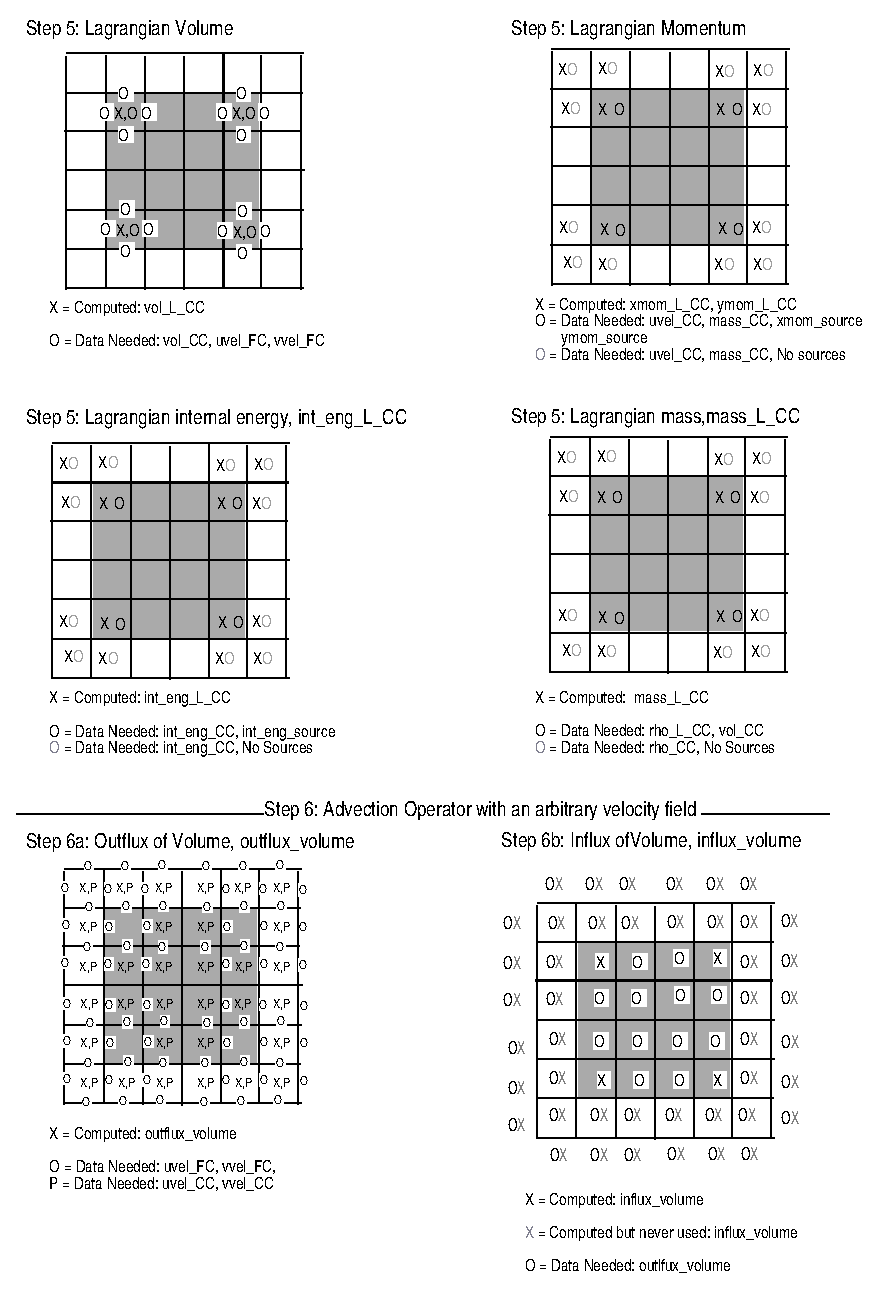
\includegraphics{boundarycond_pg2.eps}
    \caption{The dependency on ghost cell data for the computations in steps 5 - 6b}
    \label{fig:boundarycondpg2}
\end{figure}
%
%
\begin{figure}
    \center
    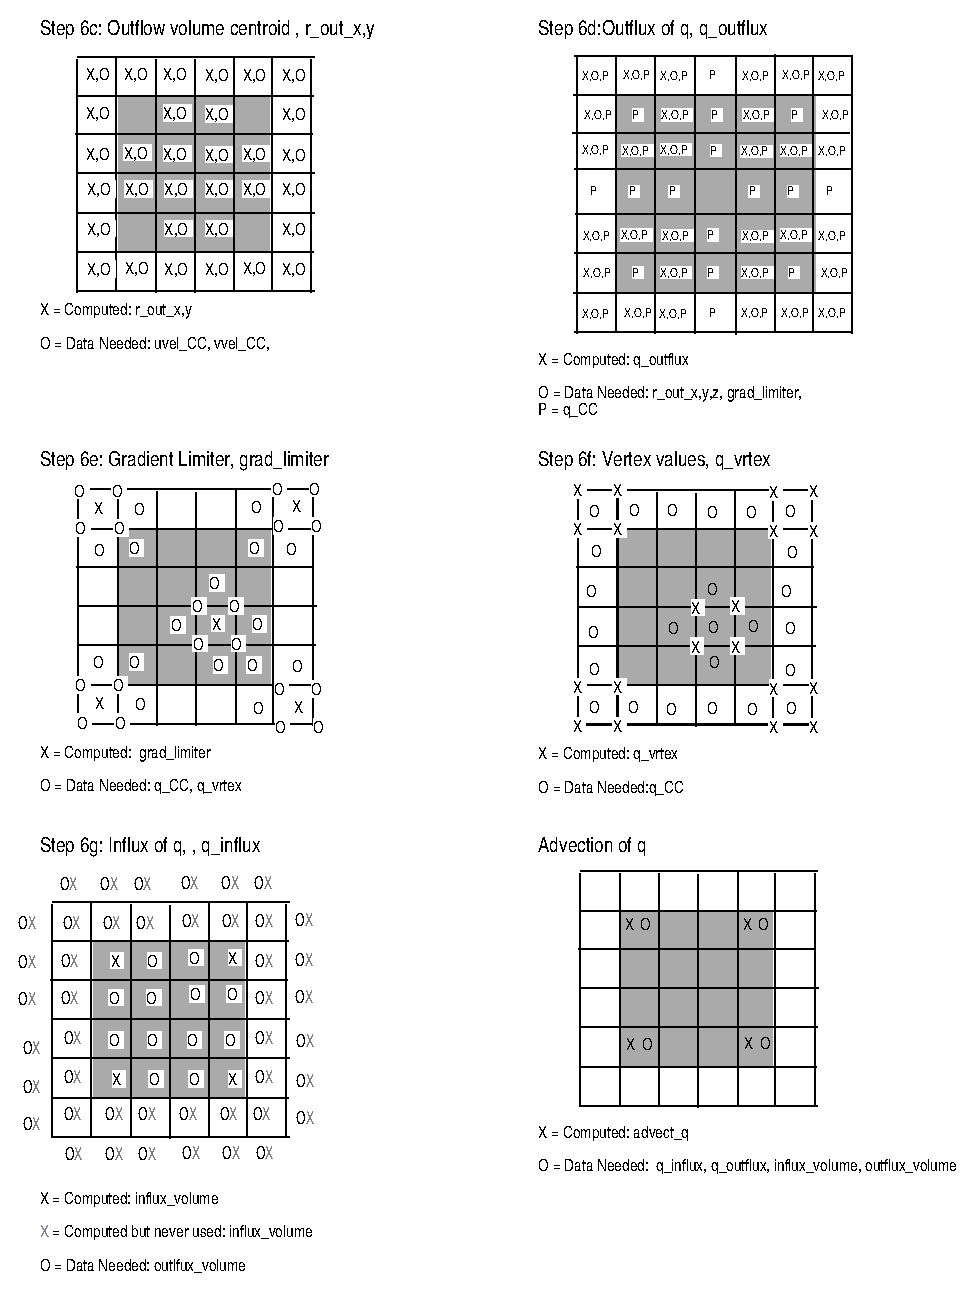
\includegraphics{boundarycond_pg3.eps}
    \caption{The dependency on ghost cell data for the computations in steps 6c - 6}
    \label{fig:boundarycondpg3}
\end{figure}
%
%
\begin{figure}
    \center
    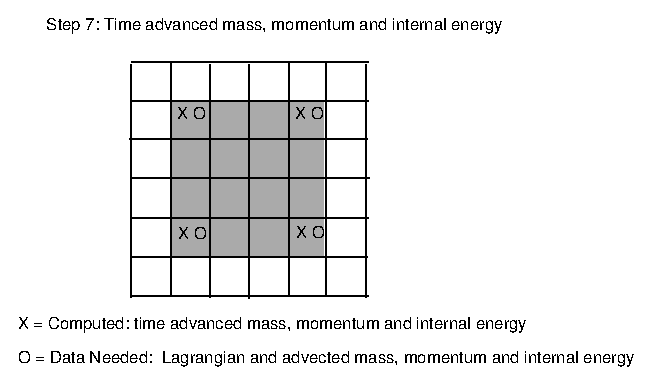
\includegraphics{boundarycond_pg4.eps}
    \caption{The dependency on ghost cell data for the computations in step 7}
    \label{fig:boundarycondpg4}
\end{figure}
%
\fi
\newpage
\bibliography{ICE_MM}
\newpage
%______________________________________________________________________
%    A  P  P  E  N  D  I  X    
%______________________________________________________________________
\section{\textsf{Appendix Derivation of the time advanced equations} }
In this section we will derive the $n+1$ time equations for the conservation
of mass, momentum and energy, eqs. 4.8 of \shortciteN{ICE}.  The goal is
to illustrate the steps that were taken from in reducing the governing
equations \ref{eq:cont_mass}~-~\ref{eq:cont_energy} to the time advanced
equations 4.6 in \shortciteN{ICE}.  In doing so we will use the right hand
side of eqs. [\ref{eq:cont_mass}~-~\ref{eq:cont_energy}]  times the volume
as the source terms.  Beginning with Reynolds transport theorem, applied to
a material volume \shortcite{thompson}.
%_______________________________
% Reynolds transport theorem
%_______________________________
\begin{equation}
    \label{eq:rey_tran2}
    \int_{V}\pd{()}{t}dV + \int_{A} ()\vec{U} \cdot d\vec{S} = \frac{d}{dt}\int_{V}()dV 
\end{equation}
%
%_______________________________
% time advanced rho
%_______________________________
Using eq. (\ref{eq:rey_tran2}) and letting $() = m_m$ the equation for the
conservation of mass for multiple materials in a control volume becomes
%
\begin{equation*}
    \int_{V}\pd{m_m }{t}dV + \int_{A} m_m \um \cdot d\vec{S} 
=   \int_{v} m_m \dot{\alpham}dV 
\end{equation*}
%
After integrating the conservation of mass becomes
% 
\begin{equation*}
    V\pd{m_m}{t}+ V\sumarea \rhom \um \cdot \vec{S} = V m_m \dot{\alpham}
\end{equation*}
%
Now replace the time derivative with a first order finite-difference
representation and rearranging
%
\begin{equation}
    \label{eq:rho}
    \boxed{
    \rhom^{n+1}V^{n+1} = \underbrace{ \delt\rhonm V^{n}  + \delt \massnm \dot{\alpham}}_{        \text{Lagrangian change in mass}  }
-   \delt \sumarea \rhonm  \unm\cdot \vec{S}}
\end{equation}
\\
%_______________________________
% time advanced momentum
%_______________________________

\underline{Momentum}
For the momentum equation we will assume that the multiphase Reynolds stress
and the acceleration by non-equilibrium pressure is zero.  If we let $()
= \rhom \um$ and substitute into eq. (\ref{eq:rey_tran2}) the momentum
equation becomes,
%
\begin{align*}
        \int_{V}\pd{\rhom \um }{t}dV + \int_{A} \rhom \um \um \cdot d\vec{S} 
&   =   \int_{V}\rho_o \vec{U}_o \dot{\alpham}dV \\
&   +   \int_{V}\rhom \vec{g}dV\\
&   +   \int_{V}\theta_m\nabla{p}dV\\
&   +   \int_{V}\nabla \cdot(\alpham \tau_o)dV\\
&   +   \int_{V}\sum_{l} \theta_k \theta_l K_{m,l}(\vec{U}_l - \um)dV
\end{align*}
%
Before this equation can be integrated we need to convert  the volume integral
for the pressure gradient and the divergence of the deformation tensor into
surface integrals.  This is done through the divergence theorem for a scalar
a tensor \shortcite{bird}
%
\[\int_{V} \nabla{s} dV = \int_A s d\vec{S}\]
\[\int_{V} \nabla \cdot{\tau} dV = \int_A \tau \cdot d\vec{S} \]
%
After making the substitution the momentum equations becomes\\
%
\begin{align*}
        \int_{V}\pd{\rhom\um }{t}dV &+ \int_{A} \rhom \um \um \cdot d\vec{S} 
=       \int_{V}\rhom \um \dot{\alpham}dV 
    +   \int_{V}\rhom \vec{g}~dV\\
&   +   \int_{A}\theta_{m} p~d\vec{S}
    +   \int_{A}\tau_m\cdot d\vec{S}
    +   V \sum_{l} \theta_k \theta_l K_{m,l}(\vec{U}_l - \um)
\end{align*}
%
We now integrate all of the terms except for those involving the pressure
and deviatoric stress tensor
%
\begin{align*}
\pd{\rhom\um }{t} &+ \sumarea \rhom \um (\um \cdot \vec{S}) 
=       m_m \um \dot{\alpham}
    +   m_m \vec{g}
    +   \int_{A}\theta_{m} p~d\vec{S}\\
&   +   \int_{A}\tau_m\cdot d\vec{S}
    +   \int_{V} \sum_{l} \theta_k \theta_l K_{m,l}(\vec{U}_l - \um)~dV
\end{align*}
%
Now replace the time derivative with a first order finite-difference
representation and rearranging\\
%
\begin{align}
(m_m\um)^{n+1}  = 
        (m_m\um)^{n}
    +   \delt \massnm \unm \dot{\alpham} 
    +   \delt m_m \vec{g}
    +   \delt \int_{A}\theta_{m} p~d\vec{S}\notag \\
    +   \delt \int_{A}\tau_m\cdot d\vec{S} 
    +   \delt V \sum_{l} \theta_k \theta_l K_{m,l}(\un_{l} - \unm)
    -   \delt \sumarea \rhom \un (\un \cdot \vec{S}) 
\end{align} 
%_______________________________
% time advanced Energy
%_______________________________
For the energy equation we start by ignoring the multiphase fluctuational
transport of internal energy, fluctuational work, average viscous
dissipation, thermal transport by conduction.  Letting $() = \rhom e_m$
in eq. (\ref{eq:rey_tran2}) the energy equation reduces to \\ %

\begin{align}
    \label{eq:j}
        \int_{V}\pd{\rhom e_m}{t}dV + \int_{A} \rhom e_m \um \cdot d\vec{S} 
&   =   \int_{V} \rho_o e_o \dot{\alpham}dV \notag \\
&   +   \int_{V}(\frac{  p_{m} \upsilon_m  }{ c^{2}_{m} }  ) \dot{p}~dV \notag\\
&   +   \int_{V} \sum_{l} \theta_k \theta_l R_{m,l}(T_l - T_m)dV
\end{align}
%
Making the substitutions
$p_k=\theta_{k}p^{o}_{k},~\dot{p}=\frac{\Delta{p}}{\delt}$ and integrating,
eq. (\ref{eq:j}) becomes
%
\begin{align*}
    \pd{m_m e_m}{t} &+ \sumarea m_m e_m (\um \cdot \vec{S})
    =   m_m e_o \dot{\alpham}
    +   V(\frac{  p_{m} \upsilon_m  }{ c^{2}_{m} }  ) \frac{\Delta{p}}{\delt}\\
&   +   V\sum_{l} \theta_k \theta_l R_{m,l}(T_l - T_m)
\end{align*}
%
Now replace the time derivative with a first order finite-difference
representation and rearranging\\
%
  \begin{align}
        (m_m e_m)^{n+1} 
&   =   (m_m e_m)^{n}
    +   \delt \massnm e_o \dot{\alpham}
    +   \delt V(\frac{  p_{m} \upsilon_m  }{ c^{2}_{m} }  ) \Delta{p} \notag\\
&   +   \delt V\sum_{l} \theta_k \theta_l R_{m,l}(T_l - T_m)
    -   \delt \sumarea \massnm \en (\um \cdot \vec{S})
  \end{align}
%
%_______________________________
% Derivation of the pressure eq 
% using the approximate projection method
%_______________________________
\subsection{Appendix: Derivation of the ``pressure equation"}
The derivation of the pressure equation begins with the Lagrangian face-centered
velocity and the equation for the pressure, \shortciteN{ICE} %

\begin{equation}
    \label{eq:append:ustar}
    \rho \frac{d \vec{U}^{f} }{dt} 
    = 
    -\nabla^{f}\pnnLc + \rho \vec{g}
\end{equation}
%
\begin{equation}
  \label{eq:append:peq}
  \frac{ dp }{ dt } 
  = 
  -\rho c^{2} \nabla \cdot \ustar
\end{equation}
%
Discretizing eqs. (\ref{eq:append:ustar} - \ref{eq:append:peq}) in time and rearranging
%
\begin{equation}
    \label{eq:append:tmp}
    \ustar - \biggl{(}\frac{\rhonc\unc}{\rhonc}\biggr{)}^f 
    = 
    -\frac{\delt}{\rho^{f}} \nabla^{f}\pnnLc + \delt\vec{g}
\end{equation}
%
\begin{equation}
    \label{eq:append:peq2}
    \nabla^{c} \cdot \ustar 
    = 
    - \frac{ \Delta{p}}{\rho \delt c^2}
\end{equation}
%

 is the time $n$ face centered velocity.  Now we take the divergence of
 equation (\ref{eq:append:tmp})
%%
\begin{equation}
    \label{eq:append:divustar2}
    \nabla^{c} \cdot \ustar  - \nabla^{c} \cdot \biggl{(}\frac{\rhonc\unc}{\rhonc}\biggr{)}^f
    = 
    -\nabla^{c} \cdot \biggl{[} \frac{\delt}{\rho^{f}}
     \nabla^{f}\pnnLc - \delt \vec{g} \biggr{]}
\end{equation}
%
%
%
Now substitute eqs. \ref{eq:append:peq2} into 
\ref{eq:append:divustar2}, multiply through by $-1$ and note that $\pnnLc = \pnc + \delpc$ and $\nabla^{c} \cdot \vec{g} = 0$
%
\begin{equation}
    \label{eq:append:temp}
     \frac{ \Delta{p}}{\rho \delt c^2} + \nabla^{c} \cdot          \biggl{(}\frac{\rhonc\unc}{\rhonc}\biggr{)}^f
    = 
    \nabla^{c} \cdot \biggl{[} \frac{\delt}{\rho^{f}}
    \nabla^{f}(\pnc + \delpc)\biggr{]}
\end{equation}
%
%
Now define an approximation to the face-centered velocity at time $n$ as
%
\begin{equation}
    \label{eq:append:uhat}
        \hat{\vec{U}}^{{n}^f} 
    =   
    \biggl{(}\frac{\rhonc\unc}{\rhonc}\biggr{)}^f
    -   \frac{\delt}{\rho^{f}}\nabla^{f}\pnc + \delt\vec{g}
\end{equation}
%
%
and its divergence is simply 
%
%
\begin{equation}
    \label{eq:append:divuhat}
    \nabla^{c} \cdot \hat{\vec{U}}^{{n}^f} 
    = 
    \nabla^{c} \cdot \biggl{(}\frac{\rhonc\unc}{\rhonc}\biggr{)}^f
    - \nabla^{c} \cdot \biggl{[}\frac{\delt}{\rho^{f}}\nabla^{f}\pnc 
    - \delt \vec{g} \biggr{]}
\end{equation}
%
%
Rearranging eq. (\ref{eq:append:temp})
\begin{equation}
    \label{eq:append:temp}
    \frac{ \Delta{p}}{\rho \delt c^2} +
    \nabla^{c} \cdot \biggl{[} \frac{\delt}{\rho^{f}}
    \nabla^{f}(\delpc)\biggr{]}
    = 
    -
    \nabla^{c} \cdot          \biggl{(}\frac{\rhonc\unc}{\rhonc}\biggr{)}^f + 
    \nabla^{c} \cdot \biggl{[} \frac{\delt}{\rho^{f}}
    \nabla^{f}(\pnc)\biggr{]}
\end{equation}

Finally we get the pressure equation
\begin{equation}
        \biggl{[}\frac{ 1}{\rho \delt c^2} 
    -   \nabla^{c} \cdot \frac{\delt}{\rho^{f}}\nabla^{f} \biggr{]} \delpc       
    =   
    -   \nabla^{c} \cdot \hat{\vec{U}}^{{n}^f}
\end{equation}
%
%
%
\newpage
%
\iffalse
%_______________________________
% Difference expressions for the gradients
%_______________________________
\subsection{Appendix: Difference Scheme}
In the ghostcells the gradients shown in eqs.(\ref{eq:discrete.qoutflux1}- \ref{eq:discrete.qoutflux4}) and (\ref{eq:vertex1} - \ref{eq:vertex4}) are computed using the following second order scheme.\\
%
\underline{Left layer of ghost cells, excluding the corner cells}
\begin{align}
    &\pd{q}{x} = \frac{-3.0 * q_{i,j,k} + 4.0 * q_{i+1,j,k} - q_{i+2,j,k}}{\delx} \notag \\
    &\pd{q}{y} = \frac{q_{j+1} - q_{j-1}}{2\dely}   \notag \\
\end{align}
%
%
\underline{Right layer of ghost cells, excluding the corner cells}
\begin{align}
    &\pd{q}{x} = \frac{3.0 * q_{i,j,k} - 4.0 * q_{i-1,j,k} + q_{i-2,j,k}}{\delx} \notag \\
    &\pd{q}{y} = \frac{q_{j+1} - q_{j-1}}{2\dely}   \notag \\
\end{align}
%
%
\underline{Top layer of ghost cells, excluding the corner cells}
\begin{align}
    &\pd{q}{x} = \frac{q_{j+1} - q_{j-1}}{2\dely}   \notag \\
    &\pd{q}{y} = \frac{3.0 * q_{i,j,k} - 4.0 * q_{i,j-1,k} + q_{i,j-2,k}}{\dely} \notag \\
\end{align}
%
%
\underline{Bottom layer of ghost cells, excluding the corner cells}
\begin{align}
    &\pd{q}{x} = \frac{q_{j+1} - q_{j-1}}{2\dely}   \notag \\
    &\pd{q}{y} = \frac{-3.0 * q_{i,j,k} + 4.0 * q_{i,j+1,k} - q_{i,j+2,k}}{\dely} \notag \\
\end{align}
%
%
For the corner ghostcells \\
\underline{Upper left ghostcell corner}
\begin{align}
    &\pd{q}{x} = \frac{-3.0 * q_{i,j,k} + 4.0 * q_{i+1,j,k} - q_{i+2,j,k}}{\delx} \notag \\
    &\pd{q}{y} = \frac{3.0 * q_{i,j,k} - 4.0 * q_{i,j-1,k} + q_{i,j-2,k}}{\dely} \notag \\
\end{align}
%
%
\underline{Upper right ghostcell corner}
\begin{align}
    &\pd{q}{x} = \frac{3.0 * q_{i,j,k} - 4.0 * q_{i-1,j,k} + q_{i-2,j,k}}{\delx} \notag \\
    &\pd{q}{y} = \frac{3.0 * q_{i,j,k} - 4.0 * q_{i,j-1,k} + q_{i,j-2,k}}{\dely} \notag \\
\end{align}
%
%
\underline{Lower right ghostcell corner}
\begin{align}
    &\pd{q}{x} = \frac{3.0 * q_{i,j,k} - 4.0 * q_{i-1,j,k} + q_{i-2,j,k}}{\delx} \notag \\
    &\pd{q}{y} = \frac{-3.0 * q_{i,j,k} + 4.0 * q_{i,j+1,k} - q_{i,j+2,k}}{\dely} \notag \\
\end{align} 
%
% 
\underline{Lower left ghostcell corner}
\begin{align}
    &\pd{q}{x} = \frac{-3.0 * q_{i,j,k} + 4.0 * q_{i+1,j,k} - q_{i+2,j,k}}{\delx} \notag \\
    &\pd{q}{y} = \frac{-3.0 * q_{i,j,k} + 4.0 * q_{i,j+1,k} - q_{i,j+2,k}}{\dely} \notag \\
\end{align} 
\fi

\end{document}
